
% Hier gibts ne Vorlage falls wir die Nutzen wollen https://git.scc.kit.edu/IPDSnelting/pflichtenheft/-/blob/master/pflichtenheft.tex
%Bindet die setup-datei ein. Beim Kompilieren wird alles was in setup.tex steht an diese stelle kopiert
%Das hier ist eine setup-Datei. hier schreiben wir Packages und setup-befehle für das Pflichtenheft rein. 
%Hält das ganze etwas übersichtlicher


%\documentclass[parskip=full,11pt,twoside]{scrartcl} - DIeses two side ist mega der bs
\documentclass[parskip=full,11pt]{scrartcl}
\usepackage[utf8]{inputenc}
\usepackage[linkcolor=blue, colorlinks=true]{hyperref}
\usepackage{glossaries}     % provides glossary commands, taken from SWT

\usepackage{svg}
\usepackage{enumitem}
\usepackage{tabularx}
\usepackage{changepage}
\usepackage{float}
\usepackage{xcolor}
% section numbers in margins:
\renewcommand\sectionlinesformat[4]{\makebox[0pt][r]{#3}#4}

% header & footer
\usepackage{scrlayer-scrpage}
\lofoot{\today}
\refoot{\today}
\pagestyle{scrheadings}


\usepackage[sfdefault,light]{roboto}
\usepackage[T1]{fontenc}
\usepackage[german]{babel}
\usepackage[yyyymmdd]{datetime} % must be after babel
\renewcommand{\dateseparator}{-} % ISO8601 date format
%usepackage[]{hyperref}
\usepackage{amsmath} % for $\text{}$
\usepackage[nameinlink]{cleveref}
\crefname{figure}{Abb}{Abb}
\usepackage[section]{placeins}
\usepackage{xcolor}
\usepackage{graphicx}
\hypersetup{
	pdftitle={Pflichtenheft},
	bookmarks=true,
}
\usepackage{csquotes}

\newcommand\urlpart[2]{$\underbrace{\text{\texttt{#1}}}_{\text{#2}}$}
\newenvironment{FA}
    {
    \begin{adjustwidth}{-3.5cm}{}
    \begin{tabular}[t]{rL{0.8\textwidth}}
    }
    {
    \end{tabular}
    \end{adjustwidth}
    \vspace{1em}
    }
    
\newenvironment{FAList}{\begin{itemize}[noitemsep, leftmargin=1cm,align=parleft]}{\end{itemize}}


\title{Pflichtenheft PSE}
\author{Valentin Schenk, Kaloyan Krasimirov Enev, Simon Wilhelm Schübel,\\ Maik Sept, Simon Aaron Giek}

\date{May 2022}
% https://en.wikibooks.org/wiki/LaTeX/Glossary

%\makenoidxglossaries
\makeglossaries

%\newglossaryentry{Job}{
%    name=Job,
%    plural=Jobs,
%    description={Jobs sind die Instanzen, die von Mallob verarbeitet werden. Ein einzelner Job stellt ein einzelnes zu lösendes Problem dar. Ein Job besteht aus Sicht des Nutzers aus der \gls{Job-Konfiguration} und der \gls{Job-Beschreibung}}
%}
%
%\newglossaryentry{Job-Konfiguration}{
%    name=Job-Konfiguration,
%    plural=Job-Konfigurationen,
%    description={
%    Die Job-Konfiguration beinhaltet alle Parameter des Jobs, welche bei der Bearbeitung berücksichtigt werden. Sie sind in den \hyperref[B:Job]{Begrifflichkeiten} näher erläutert
%    }
%}
%
%\newglossaryentry{Job-Beschreibung}{
%    name=Job-Beschreibung,
%    plural=Job-Beschreibungen,
%    description={Die Job-Beschreibung ist der Teil des Jobs, der das eigentliche Problem darstellt}
%}
%
%\newglossaryentry{Job-Informationen}{
%    name=Job-Informationen,
%    description={Die Job-Informationen enthalten die \gls{Job-Konfiguration} und den Einreiche-Zeitpunkt, den Zustand des Jobs, die Informationen die Mallob über den Job bereitstellt und die Job-ID. Sie enthält nicht die Job-Beschreibung und nicht das rohe Ergebnis des Jobs}
%}
%
%\newglossaryentry{Job-Updates}{
%    name=Job-Updates,
%    description={Job-Updates sind jene Informationen eines Jobs, die für die Visualisierung des Systems benötigt werden. Dazu gehören die Informationen, wie Mallob den Job gerade auf die Kerne verteilt hat und wie sich der \gls{Binaerbaum} des Jobs verändert}
%}


\newglossaryentry{Nutzer}{
    name=Nutzer,
    plural=Nutzer,
    description={Ein Nutzer ist eine Person, welche sich registriert hat und die mit dem System interagiert}
}


\newglossaryentry{Nutzerkonto}{
    name=Nutzerkonto,
    plural=Nutzerkonten,
    description={Ein Nutzerkonto ist ein im System durch einen Nutzer registriertes und durch einen Administrator verifiziertes Konto}
}

\newglossaryentry{Administrator}{
    name=Administrator,
    plural=Administratoren,
    description={Administratoren sind Nutzer mit mehr Rechten zur Verwaltung des Systems. Sie haben dennoch alle Möglichkeiten, die auch ein Nutzer hat, welcher kein Administrator ist}
}

\newglossaryentry{Web-Interface}{
    name=Web-Interface,
    description={Mit Web-Interface wird die Webseite von \textit{Fallob} referenziert, die der Nutzer im Internet aufrufen kann}
}
\newglossaryentry{API}{
    name=API,
    plural=APIs,
    description={Application Programming Interface. Wird im Kontext dieses Systems genutzt, um die Dienste in einer Art und Weise bereitszustellen, dass sie in andere Anwendungen integriert werden kann}
}

\newglossaryentry{Konfigurationsdatei}{
    name=Konfigurationsdatei,
    description={Eine Datei in einem spezifischen Format, die vom System eingelesen wird. Darin werden bestimmte Werte definiert, die dann vom System verwendet werden}
}
\newglossaryentry{System-Administrator}{
    name=System-Administrator,
    description={Eine Person, die die Ausführungsumgebung des Systems verwaltet. Verantwortlich für das Starten und Beenden des Systems}
}

\newglossaryentry{Authentifizierungstoken}{
    name=Authentifizierungstoken,
    description={Ein Token (sog. Bearer-Token), kann benutzt werden, um sich gegenüber einer API zu authentifizieren. Der Token verweist auf nur genau einen Nutzer. Dieser Token kann von jedem benutzt werden, der ihn besitzt (deswegen Bearer-Token). Der Token wird für jeden Nutzer bei der Registrierung generiert, sodass niemals zwei Nutzer denselben Token haben. Für den Nutzer ist es wichtig den Token, wie seine Anmeldedaten, geheim zu halten, bzw. nur authorisierten Personen mitzuteilen}
}

%\newglossaryentry{Anfrage}{
%    name=Anfrage
%    plural=Anfragen
%    description={Ein Nutzer kann eine Anfrage an eine API oder eine Website stellen.}
%}

\newglossaryentry{Datenbank}{
    name=Datenbank,
    plural=Datenbanken,
    description={Eine Datenbank ist ein System, welches zur Datenspeicherung und Verwaltung genutzt wird. Die Hauptaufgabe einer Datenbank besteht darin, vordefinierte Daten zu speichern und schnellen Zugriff auf die Daten zu erlangen}
}

\newglossaryentry{Output-Log}{
    name=Output-Log,
    description={}
    }

\newglossaryentry{Stream}{
    name=Stream,
    description={Ein Stream von Daten ist eine andauernde eingehende oder ausgehende Menge von Daten}
}

\newglossaryentry{Log-Datei}{
    name=Log-Datei,
    description={Eine Log-Datei ist eine Datei, welche Log-Daten speichert. Log-Daten sind Meta-Daten, welche gewisse Ereignisse festhalten sollen. Im Kontext von Mallob beispielsweise das Eingehen eines Jobs}
}

\newglossaryentry{Vorlaeufiges Nutzerkonto}{
    name={Vorläufiges Konto},
    description={Ein vorläufiges Konto sind Konten, die neu erstellt wurden und noch nicht durch einen \gls{Administrator} verifiziert wurden. Ein solches Konto eingeschränkt, es könnten noch keine Jobs in Auftrag gegeben werden}
}

    
\newglossaryentry{Bearbeitungszeit}{
name=Bearbeitungszeit,
description= {tt}%[todo]
}


\newglossaryentry{Dropdown-Menue}{
    name=Dropdown-Menü,
    plural=Dropdown-Menüs,
    description={Das Dropdown-Menü ist eine spezielle Form eines Auswahlmenüs. Nach dem Klick auf einen entsprechenden Button oder durch die Berührung mit dem Mauszeiger erscheint eine Auswahlliste auf dem Bildschirm. Durch einen weiteren Klick auf den gewünschten Menüpunkt wird dieser aufgerufen}
}

\newglossaryentry{URL}{
    name=URL,
    plural=URLs,
    description={Die URL (Uniform Resource Locator) ist die Adresse einer einzelnen Webseite}
}


%--------------neue glossareinträge ab 26.05.2022

\newglossaryentry{Checkbox}{
    name=Checkbox,
    plural={Checkboxen},
    description={Eine Checkbox ist ein Kästchen, welches 'gecheckt' werden kann, also betätigt oder nicht betätigt. Im falle des clickens einer Checkbox wird ein Haken in die Checkbox gesetzt (die Checkbox ist bestätigt), welcher bestehen bleibt, bis die checkbox ein weiteres mal geklickt wird (Checkbox ist nicht mehr bestätigt)}
}

\newglossaryentry{Nutzername}{
    name=Nutzername,
    plural=Nutzernamen,
    description={Der Nutzername ist derjenige Name, mit dem sich ein \gls{Nutzer} im System registriert und mit dem er auch referenziert wird.}
}


\newglossaryentry{Model-View-Controller}{
    name=Model-View-Controller,
    description={Model-View-Controller beschreibt ein Konzept aus der Softwaretechnik, nachdem eine Software in drei Komponenten aufgeteilt wird}
    }
    
\newglossaryentry{API-Anfrage}{
    name= API-Anfrage,
    description={Eine API-Anfrage ist die Benutzung der API durch einen Nutzer}%TODO : was??
}

\newglossaryentry{Testueberdeckung}{
    name=Testüberdeckung,
    plural=Testüberdeckungen,
    description={Die Testüberdeckung eines Programmes beschreibt den prozentualen Anteil der Codezeilen, die durch mindestens einen Testfall überprüft werden}
}


\newglossaryentry{Betriebssystem}{
    name=Betriebssystem,
    plural=Betriebssysteme,
    description={Ein Betriebssystem ist eine Software, die eine Schnittstelle zwischen der Hard- und Software des Computers herstellt und das Ausführen von Programmen ermöglicht}
}

\newglossaryentry{k-Means}{
    name={k-Means},
    description={Ein k-Means Algorithmus ist ein verfahren zur Vektorquantisierung, das auch zur Clusteranalyse verwendet wird. Dabei wird aus einer Menge von ähnlichen Objekten eine vorher bekannte Anzahl von k Gruppen gebildet}
}

\newglossaryentry{SAT}{
    name=SAT,
    description={SAT steht für Statisfyability und beschreibt ein NP-Schweres Problem. Eine SAT-Probleminstanz besteht aus einer Klauselmenge $C$ und einer Variablenmenge $V$. Eine Erfüllende Lösung für eine SAT-Instanz weißt jeder Variable $v \in V$ eine Belegung $b \in \{0,1\}$ zu, sodass alle Klauseln erfüllt sind}
}

\newglossaryentry{NP-schweres Problem}{
    name={NP-schweres Problem},
    plural={NP-schwere Probleme},
    description={NP-Schwere bezeichnet die Eigenschaft eines algorithmischen Problems, mindestens so schwer lösbar zu sein, wie die Probleme der Klasse NP. Die Klasse NP beinhaltet Probleme, für deren Lösung keine Algorithmen in Polynomialzeit bekannt sind} 
}


\newglossaryentry{Versionsverwaltung}{
    name=Versionsverwaltung,
    plural=Versionsverwaltungen,
    description={Eine Versionsverwaltung ist ein Programm, das zur Erfassung von Änderungen an Dokumenten oder Dateien verwendet wird. Es ist somit möglich, Änderungen rückgängig zu machen und alte Versionen wiederherzustellen}
}

\newglossaryentry{Systemzustand}{
    name=Systemzustand,
    description={Der Systemzustand beschreibt die Aktuelle Einstellung des Systems. Jede Einstellung, jede gespiecherte Variable}
}

\newglossaryentry{Prozess}{
    name=Prozess,
    plural=Prozesse,
    description={Ein Prozess, auch Programminstanz genannt, ist ein Computerprogramm zur Laufzeit. Genauer ist ein Prozess die konkrete Instanziierung eines Programms}
}

\newglossaryentry{Binaerbaum}{
    name={Binärbaum},
    plural={Binärbäume},
    description={Ein Binärbaum ist, im Sinne der Graphentheorie, ein zusammenhängender, kreisfreier Graph, welcher für jeden Knoten höchstens Ausgansgrad 2 aufweist. In unserem Fall sprechen wir speziell von balancierten Binär-Bäumen, dass heißt, dass die Höhe des Baumes (die maximal mögliche Länge eines Weges, der in der Wurzel endet), durch $c*log(n)$ beschränkt ist (dabei ist $c$ eine Konstante und $n$ die Anzahl der Elemente im Baum)}
}

\newglossaryentry{Teilbaum}{
    name={Teilbaum},
    plural={Binär-Bäume},
    description={Ein Teilbaum ist, im Sinne der Graphentheorie, ein Baum, dessen Wurzel ein Konten eines anderen Baumes ist}
}


\newglossaryentry{Plugin}{
    name=Plugin, 
    plural=Plugins,
    description={Ein Plug-In ist ein Softwareprogramm, auf das von anderen Softwareanwendungen zugegriffen werden kann, um deren Funktionalität zu erweitern}
}

\begin{document}

\newcolumntype{L}[1]{>{\raggedright\arraybackslash}p{#1}}
\newcolumntype{C}[1]{>{\centering\arraybackslash}p{#1}}
\newcolumntype{R}[1]{>{\raggedleft\arraybackslash}p{#1}}


\maketitle
\newpage
\tableofcontents 
\newpage
\section{Einleitung}


%Neben der
%-expliziten Benennung des Auftragnehmers und des Auftraggebers 
%sollte an dieser Stellung auch eine 
%-grobe Kurzbeschreibung des Projektes erfolgen. 
%Gehen Sie darauf ein, 
%--was das Projekt beinhaltet und 
%--wie das Endergebnis aussehen soll. 
%Wichtig ist, dass auch eine Person, die das erste Mal von dem Projekt hört, versteht, worum es geht.

%---Vorstellung des Auftraggebers und von uns 
Mallob ist ein dezentrales System zur Lösung von NP-schweren Problemen, hauptsächlich entwickelt von Dominik Schreiber im Rahmen seiner Doktorarbeit. Der Auftraggeber - die Entwickler von Mallob - wünschen sich von 5 randoms eine [bedienerfreundliche Möglichkeit, Schnittstelle, Interface], um mit Mallob von außen kommunizieren zu können.\\

%---Grobe kruzbeschreibung des Projekts
Unser System - \textbf{a friendly face for Mallob} - soll diese Brücke zwischen Mallob und Außenwelt darstellen. 

Es verfügt daher über all diejenigen Funktionen, die es möglich machen mit Mallob zu interagieren. Es ist also möglich direkt Aufträge an Mallob zu stellen und Informationen über diese zu erlangen.

Eine Hauptaufgabe des friendly faces ist die Echtzeit-Visualisierung der Arbeitsweise von Mallob. Hier ist es möglich zu sehen wie Mallob die eigenen Jobs (so werden Probleme genannt, die Mallob lösen soll) bearbeitet. Auch die Gesamtauslastung sowie Arbeitsweise ist einsehbar. 

Die Interaktion mit Mallob soll sowohl über ein Web-Interface, als auch direkt über eine von uns bereitgestellte API möglich sein. %\\

%Des weiteren wird das System eine Nutzer-Verwaltung beinhalten, um %[warum haben wir eine Nutzerverwaltung?]. 

\newpage
%\section{Zielbestimmung}
%\subsection{Musskriterien}
%\subsubsection{Web-Interface}
%\begin{itemize}
%    \item Das System verfügt über ein \gls{Web-Interface}.
%    \item Beim ersten Aufruf des \glslink{Web-Interface}{Web-Interfaces} wird eine Anmelde-Maske angezeigt.
%    \item In der Anmelde-Maske der Nutzer auch zu einer Maske für die Registierung gelangen.
%    \item Ein \gls{Auftrag} kann über das \gls{Web-Interface} hinzugefügt werden. Dies geschieht über eine Eingabemaske.
%    \item Das Übergeben der Probleminstanz kann wahlweise direkt über ein Eingabefeld, hochladen der CNF-Datei oder Angabe einer URL erfolgen.
%    \item Das \gls{Web-Interface} besitzt eine Visualierung des Systemzustandes. Hier wird standardmäßig der aktuelle Zustand visualisiert,  es kann aber auch die Historie betrachtet werden.
%    \item Admins haben Zugriff auf eine exklusive Ansicht, mit der die Instanz von Mallob verwaltet werden kann.
%
%\subsection{Wunschkriterien}
%\subsubsection{Web-Interface}
%\begin{itemize}
%    \item Der Benutzer kann die Eingabe des Problems mit einem graphischem Editor vornehmen.
%    \item Ein Admin kann die Instanz von Mallob starten, beenden und neustarten. Hier gibt es auch die Möglichkeit, entsprechende Parameter einzugeben.
%\end{itemize}
%\end{itemize}

\section{Zielbestimmung}
\textit{Fallob} ermöglicht es Nutzern, einfacher mit \href{https://github.com/domschrei/mallob}{Mallob} zu interagieren. Diese Interaktion kann auf zwei Wege erfolgen:
Einerseits wird eine REST-API für die Interaktion angeboten. Anderseits gibt es aber auch ein benutzerfreundliches Web-Interface, welches die API nutzt und somit eine graphische Oberfläche für diese darstellt. Auf beide Wege können eigene Jobs verwaltet werden. Darüber hinaus bietet das Web-Interface auch eine Visualisierung des Systems.


\subsection{Musskriterien}
    \subsubsection{API}
        \begin{itemize}[noitemsep]
            \item Authentifizieren von Nutzern
            %\item Registrieren von neuen Nutzer
            \item Job einreichen
            \item Job abbrechen
            \item Informationen zu Jobs abfragen
            \item Ergebnis von Jobs abfragen
            \item Beschreibung von Jobs abfragen
            \item Bereitstellung eines Ereignis-Streams von Mallob zum Erhalten von Updates von Jobs
            \item Abfrage des Status der Mallob-Instanz
            %\item Erhalten von Informationen zu aufgetretenen Fehlern
        \end{itemize}
    \subsubsection{Web-Interface}
        \begin{itemize}[noitemsep]
            \item Authentifizieren von Nutzern
            %\item Registrierung von neuen Nutzern
            \item Tabellarische Übersicht  der Jobs
                \begin{itemize}[noitemsep]
                    \item Abbrechen mehrerer Jobs auf einmal
                    \item Herunterladen von mehreren Ergebnissen auf einmal
                \end{itemize}
            \item Job über Eingabemaske einreichen
                \begin{itemize}[noitemsep]
                    \item Einreichen der Job-Beschreibung über ein Eingabe-Feld
                    \item Einreichen der Job-Beschreibung durch Hochladen einer entsprechenden Datei
                \end{itemize}
            \item Job abbrechen
            \item Aktuellen Status des Jobs betrachten
            \item Job-Seite um Details von Jobs anzusehen
            \item Herunterladen der Ergebnisse der Jobs
            \item Anzeigen von aufgetretenen Fehlern bei Nutzern
            \item Anzeigen von Warnungen von Mallob im Administratoren-Bereich 
            %\item Verifizierungsmöglichkeit von neuen Nutzern für Administratoren 
            
                      
        \end{itemize}
    \subsubsection{Visualisierung}    
        \begin{itemize}[noitemsep]
            \item Das Web-Interface enthält eine Visualisierung des System-Zustands
                \begin{itemize}[noitemsep]
                    \item Darstellung der Prozesse als Punkte, ein Punkt je Prozess %TODO: Ranks? oder PEs? oder ganz anderes Word?
                    \item Färbung der Punkte entsprechend dem zugehörigen Job
                    \item Verbinden der Punkte entsprechend der Position im Binärbaum des Jobs
                    \item Dynamische Größe der Punkte und Verbindungen entsprechend der Position im Binärbaum des Jobs
                \end{itemize}
            \item Automatische Aktualisierung der Visualisierung, wenn die Live-Ansicht ausgewählt ist
            %\item Wenn die Live-Ansicht ausgewählt ist, wird die Visualisierung automatisch aktualisiert
            \item Darstellen eines bestimmten vergangenen Zeitpunktes
            \item Ändern der Wiedergabegeschwindigkeit
            \item Einsehen von Details zu einem aktiven Job in einem separatem Feld 
            %\item Darstellung der PE als Punkte %TODO: Ranks? oder PEs? oder ganz anderes Word?
            %\item Färbung der Punkte entsprechend dem zugehörigen Job
            %\item Verbinden der Punkte entsprechend der Position im Binärbaum des Jobs
            %\item Dynamische Größe der Punkte und Verbindungen entsprechend der Position im Binärbaum des Jobs.
        \end{itemize}
    
    \subsubsection{System}
        \begin{itemize}[noitemsep]
            \item Konfigurationsdatei für globale Einstellungen des Systems
        \end{itemize}
        
        
\subsection{Wunschkriterien}
    \begin{itemize}[noitemsep]
        %\item Speichern von Jobdaten für Statistiken -> Irgendwie redundaten, da wir eh schon jobdaten speichern
        \item Möglichkeit für Administratoren, Mallob zu starten, beenden oder neuzustarten
        \item Registrierung von Nutzern über die API
        \item Registrierung von Nutzern über das Web-Interface
        \item Sortieren der Job-Tabelle im Web-Interface
        \item Möglichkeit zum Neustart von abgebrochenen oder abgeschlossenen Jobs
        \item Eingabemaske für die Eingabe der Job-Beschreibung im Web-Interface
        \item Einreichen der Job-Beschreibung über eine URL, die auf die Job-Beschreibung zeigt
        \item Diagnosemöglichkeit für Administratoren im Web-Interface
        \item Nutzer benachrichtigen, falls Mallob abstürzen sollte
        \item Darstellung des vollständigen Binärbaums des Jobs in der Visualisierung
        \item Schnittstelle für Plugins in Web-Interface
        \item Entwicklung eines beispielhaften Plugins
    \end{itemize}
    
\subsection{Abgrenzungskriterien}
    \begin{itemize}[noitemsep]
        \item Es kann maximal ein Auftrag pro Anfrage hinzugefügt werden
        \item Korrektheit der Daten wird durch Mallob geprüft
        \item Es gibt keine Möglichkeit, falsche Daten in der API zu korrigieren, in diesem Fall muss die gleiche Anfrage mit korrekten Daten erneut erfolgen
    \end{itemize}

\newpage
\section{Produkteinsatz}
% TODO: das sollte noch mindestens zwei mal überarbeitet werden, lol

\subsection{Andwendungsbereich}

Das System dient dem Lösen von Problemen. Ein Nutzer kann das Web-Interface im Browser aufrufen oder stattdessen die bereitgestellte API nutzen.
\subsection{Zielgruppe}

Insgesamt richtet sich das System an Personen, die komplexe Probleme lösen möchten, deren Laufzeit zu groß ist. Hier kann dieses System helfen, indem es das Problem schneller löst. 
Das Web-Interface bietet eine moderne, einfach und intuitive Umgebung zur Nutzung dieses Systems. Hier sind abgesehen von der Bereitstellung der Job-Beschreibung im korrekten Format keine weiteren Kenntnisse notwendig. \\
Die API dagegen richtet sich an Personen, die dieses System in ihr eigenes integrieren möchten. Hier wird Wissen über den Umgang einer solchen API vorausgesetzt. 
\subsection{Betriebsbedingungen}

\begin{itemize}
    \item Zur Nutzung ist eine stabile Internetverbindung notwendig. Insbesondere kann eine instabile Verbindung dazu führen, das Ereignisse nicht in Echtzeit angezeigt werden.
    \item Zur Verwendung des Web-Interfaces muss ein aktuelle Version des Browsers genutzt werden.
    \item Das System muss Zugriff auf die API der Instanz von Mallob haben.
    \item Eine Instanz von Mallob muss existieren, sodass diese von diesem System genutzt werden kann. 
\end{itemize}
\newpage
\section{Produktumgebung}
\newpage
%\section{Funktionale Anforderungen}
% Sollten wir noch nutzen
%https://de.overleaf.com/learn/latex/Cross_referencing_sections%2C_equations_and_floats


\subsection{API}

\begin{itemize}
    \item[FA10] \textbf{Registrierung von Nutzern} \\
    Es ist möglich neue Nutzer über die API zu registrieren, sodass diese sich mit ihren Zugangsdaten authentifizieren können.
    
    \item[FA20] \textbf{Authentifizierung von Nutzern} \\
    Nach dem Registrieren ist es dem Nutzer möglich sich über die API zu authentifizieren und Zugriff auf die anderen Funktionen der API zu erlangen. Dies kann er mit seinem Bearer-Token tun. Diesen Token erhält ein Nutzer bei Registrierung.
    
    \item[FA30] \textbf{Einreichen von Jobs} \\
    Die API ermöglicht es Jobs, die durch eine JSON-Datei und eine Job-Beschreibung spezifiziert werden, zu übergeben. Es existieren drei verschiedene Möglichkeiten um die Job-Beschreibung zu übergeben. Die Jobs werden von Mallob bearbeitet und das Ergebnis wird an den Nutzer zurückgegeben.
    %genaue Spezifizierung der Jobs (Priorität,Laufzeit, ...) auch hier oder an anderer Stelle?
    
    \begin{itemize}
        \item[FA31] \textbf{Einreichen der Job-Beschreibung separat von der JSON-Datei} \\
        Es ist möglich die Job-Beschreibung in einer eigenen Datei zu spezifizieren. Dabei muss es sich um eine Datei handeln, die dem DIMACS CNF Standard entspricht. Diese Datei wird zusammen mit der JSON-Datei an die API übergeben.
        % soll das Dateiformat überhaupt hier schon spezifiziert werden?
        
        \item[FA32] \textbf{Job-Beschreibung innerhalb der JSON-Datei} \\
        Es ist möglich die Job-Beschreibung direkt in der JSON-Datei zu spezifizieren. Die Beschreibung muss auch in diesem Fall dem DIMACS CNF Format entsprechen. Bei dieser Möglichkeit wird nur die JSON-Datei an die API übergeben
        
        \item[FA33] \textbf{Übergeben der Job-Beschreibung über einen Link} \\
        Es kann ein Link an die API übergeben werden, der auf eine Datei verweist, in der die Job-Beschreibung enthalten ist. Die referenzierte Datei muss ebenfalls dem DIMACS CNF Format entsprechen. Zusätzlich zu dem Link muss die JSON-Datei mit den weiteren Job-Spezifikationen an die API übergeben werden
        
        \item[FA34] \textbf{Bereits eingereichte Job-Beschreibung verwenden}\\
        Ein Nutzer kann Job-Beschreibungen, welche er Bereits eingereicht hat über eine ID referenzieren und wiederverwenden.
        
    \end{itemize}
    
    \item[FA40] \textbf{Abbrechen von eingereichten Jobs} \\
    Der Nutzer kann einen eingereichten Job wieder abbrechen. In diesem Fall wird eine Statistik über die bereits verrichtete Arbeit zurückgegeben.
    
    \item[FA50] \textbf{Zurückgeben von Ergebnissen} \\
    Für jeden eingereichten Job gibt die API immer eine Antwort an den Nutzer zurück. 
    
    \begin{itemize}
        \item[F51] \textbf{Zurückgeben des Ergebnisses bei erfolgreicher Berechnung} \\
        Wurde der eingereichte Job erfolgreich gelöst, wird das Ergebnis des Jobs an den Nutzer zurückgegeben.
        
        \item[F52] \textbf{Zurückgeben des Ergebnisses nach Erreichen der maximalen Bearbeitungszeit} \\
        Wenn die maximale Bearbeitungszeit des eingereichten Jobs erreicht wurde und kein Ergebnis gefunden wurde, wird eine Statistik über die bereits verrichtete Arbeit an den Nutzer zurückgegeben
        
        \item[F53] \textbf{Zurückgeben des Ergebnisses nach einem Fehler} \\
        Wenn während der Bearbeitung des eingereichten Jobs ein Fehler auftritt, wird eine aussagekräftige Fehlermeldung an den Nutzer zurückgegeben
        
        \item[FA54] \textbf{Ergebnisabfrage von Jobs} \\
        Es ist möglich für jeden Job (auch nach Beendigung) seinen aktuellen Status (in Bearbeitung, Bearbeitet, Fehler) abzufragen. Die Antwort  enthält dabei alle Informationen zum Status des Jobs, wie das Ergebnis oder eventuelle Fehlermeldung.
    \end{itemize}
    

    \item[FA60] \textbf{Zurückgeben des Systemzustands von Mallob} \\
    
    

\end{itemize}


%------------------------------------------------------------WEB-Interface
\subsection{Web-Interface}



% Web-Interface nochmal anders formuliert, eher an Beispiel von Betreuern orrientiert
\begin{itemize}
     \item[FA010] \textbf{Web-Interface aufrufen} \\
        Nach dem Aufrufen des Web-Interface über die URL gelangt man zur Anmelde-Maske.

     \item[FA020] \textbf{Anmelden} \\
        Der Nutzer kann sich über das Web-Interface anmelden. Dies geschieht über die Anmelde-Maske. Die Anmeldung geschieht mit Nutzernamen und Passwort. Nach erfolgreicher Registierung wird der Nutzer zur Auftrag-Seite gebracht.
        
     \item[FA030] \textbf{Registrieren} \\
        Der Nutzer kann sich über das Web-Interface registrieren. Dies geschieht über die Registrieren-Maske. Diese kann von der Anmelde-Maske mit der entsprechenden Schaltfläche erreicht werden. 
        
    \begin{itemize}
        \item[FA031] \textbf{Daten zur Registrierung} \\
        Für die Registrierung wird ein Nutzername, ein Passwort und die wiederholte Eingabe des Passworts benötigt. Nach erfolgreicher Registierung wird der Nutzer zur Auftrag-Seite gebracht.
    \end{itemize}
        

        
    \item[FA040] \textbf{Ergebnisse einsehen} \\
        Befindet sich in der Liste der Aufträge ein abgeschlossener Auftrag, so kann über die zu diesem Auftrag gehörige Schaltfläche "get results" das Ergebnis angezeigt werden. Hier kann es auch in die Zwischenablage kopiert werden oder heruntergeladen werden.
        
   \item[FA050] \textbf{Auftrag hinzufügen} \\ 
        Mittels einer Schaltfläche über der Liste der eigenen Aufträge gelangt der Nutzer zu einer Eingabe-Maske, über welche er einen neuen Auftrag hinzufügen kann. 
   \item[FA00] \textbf{Auftrag abbrechen} \\
   
   \item[FA070] \textbf{Anzeigen von Fehlern} \\
        Tritt bei Mallob ein Fehler auf, so wird der Nutzer umgehend mittels einer Fehlermeldung darauf aufmerksam gemacht. Diese Fehlermeldung wird immer angezeigt, unabhängig davon auf welcher Seite der Nutzer sich momentan befindet. 
    \item[FA080] \textbf{Visualisierung} \\
        Das Web-Interface besitzt eine Visualisierung des System-Zustandes. Diese kann über den entsprechenden Reiter erreicht werden.
        
        \begin{itemize}
            \item[FA081] \textbf{Anzeigen des aktuellen Zustandes} \\
                Standardmäßig wird immer der aktuelle Zustand angezeigt. Dieser Zustand wird, solange kein anderer Zeitpunkt ausgewählt wurde, steht dynamisch aktuell gehalten. 
            \item[FA082] \textbf{Zeitachse} \\
                Die Visualisierung verfügt über eine Zeitachse, mit derer ein entsprechender Zeitpunkt der letzten [...] Minuten/Stunden ausgewählt werden kann. Nach der Auswahl wird der System-Zustand zum entsprechenden Zeitpunkt angezeigt.
            \item[FA083] \textbf{Zurückspringen zu aktueller Ansicht} \\
                Wird mittels FA71 [TODO: REF] der angezeigte Zeitpunkt geändert, so wird eine Schaltfläche angezeigt, mit der der Nutzer jederzeit wieder zur aktuellen Zeit zurückspringen kann.
            \item[FA084] \textbf{Einsehen der Verteilung eines Auftrages} \\
                 
        \end{itemize}
    \item[FA090] \textbf{Ändern von Benutzer-Daten} \\
    
    \item[FA100] \textbf{Verwalten von Nutzern}
    \item[FA110] \textbf{Verwalten von Nutzern}
        \begin{itemize}
            \item Nutzer löschen
            \item Nutzer verifizieren [TODO: besseres Wort für freigeben, ich meine damit das das der Admin den Nutzer eben bestätigen muss, bevor er Aufträge hinzufügen kann...j]
            \item 
        \end{itemize} 
    \item[FA120] \textbf{Abmelden} \\
        Der Nutzer kann sich jederzeit über das entsprechende Menü in der Navigationsleiste abmelden. In diesem Falle wird wieder die Anmelde-Maske angezeigt.
\end{itemize}




\subsection{Plugins}
\section{Nichtfunktionale Anforderungen}

\section{Funktionale Anforderungen}
% Sollten wir noch nutzen
%https://de.overleaf.com/learn/latex/Cross_referencing_sections%2C_equations_and_floats

%Produktanforderungen nach dem Stil in SWT


%Vorlange für Funktionale Anforderungen, Orientierung
%\item[F10] \textbf{Registrierung von Nutzern} \\
%    \begin{FA}
%        \textbf{Vorbedingung:} &  -keine- \\
%        \textbf{Nachbedingung (Erfolg):} &  der Nutzer besitzt einen Authentifizierungstoken für die API\\
%        \textbf{Nachbedingung (Fehlschlag):} &  der Nutzer besitzt keinen Authentifizierungstoken für die API \\
%        \textbf{Akteure:} & Nutzer, Administrator\\
%        \textbf{Auslösendes Ereignis:} & Nutzer möchte API verwenden \\
%    \end{FA}
%    \textbf{Beschreibung:}
%    \begin{FAList} 
%        \item[1.] Der Nutzer schickt eine Anfrage mit seinen Nutzerdaten an die API
%        \item[2.] Die Anfrage wird von einem Administrator bearbeitet 
%        \item[3.] Der Authentifizierungstoken wird an den Nutzer zurückgegeben
%    \end{FAList}
%    
%    
%Vorlange für Funktionale Anforderungen, zum Einfügen von Text
%\item[F10] \textbf{} \\
%    \begin{FA}
%        \textbf{Ziel:} &  \\
%        \textbf{Vorbedingung:} &  \\
%        \textbf{Nachbedingung (Erfolg):} &  \\
%        \textbf{Nachbedingung (Fehlschlag):} &   \\
%        \textbf{Akteure:} & \\
%        \textbf{Auslösendes Ereignis:} &  \\
%    \end{FA}
%    \textbf{Beschreibung:}
%    \begin{FAList} 
%        \item[1.] 
%        \item[2.] 
%        \item[3.] 
%    \end{FAList}

\subsection{API}


\begin{itemize}[nosep]
    \setlength\itemsep{4em}
  
    %-----------------API - Authentifizierung von Nutzern
    \phantomsection
    \label{FA:API:Authentifizieren von Nutzern}
    \item[F1010] \textbf{Authentifizieren von Nutzern}\\
    
    \begin{FA}
        \textbf{Ziel:} & Ein Nutzer kann sich mit seinem Nutzernamen und Passwort authentifizieren \\
        \textbf{Vorbedingung:} & Der Nutzer registriert (siehe F10) \\
        \textbf{Nachbedingung (Erfolg):} & Der Nutzer hat einen Authentifizierungstoken, der ihm Zugriff auf die Funktionen der API ermöglicht \\
        \textbf{Nachbedingung (Fehlschlag):} & Der Nutzer hat keinen Authentifizierungstoken und hat eine Fehlermeldung erhalten \\
         \textbf{Akteure:} & Nutzer \\
        \textbf{Auslösendes Ereignis:} & Nutzer möchte Funktionen der API verwenden \\
    \end{FA}
    \textbf{Beschreibung:}
    \begin{FAList}
        \item[1.] Der Nutzer schickt eine Anfrage zur Authentifizierung an die API, die seinen Nutzernamen und sein Passwort enthält
        \item[2.] Die Anfrage wird von der API verarbeitet und der Nutzer wird authentifiziert
        \item[3.a.] Wenn die Authentifizierung erfolgreich war, wird der Authentifizierungstoken an den Nutzer zurückgegeben
        \item[3.b.] Wenn die Authentifizierung nicht erfolgreich war, wird eine Fehlermeldung an den Nutzer zurückgegeben
    \end{FAList}
    
    

    
    %-----------------API - Einreichen von Jobs
    \phantomsection
    \label{FA:API:Einreichen von Jobs} 
    \item[F1020] \textbf{Einreichen von Jobs} \\
    \begin{FA}
        \textbf{Ziel:} & Ein Nutzer kann einen Job an die API übergeben, der von Mallob bearbeitet wird \\
        \textbf{Vorbedingung:} & Der Nutzer hat sich mittels \hyperref[FA:API:Authentifizieren von Nutzern]{F1010} authentifiziert \\
        \textbf{Nachbedingung (Erfolg):} & Der Nutzer hat das Ergebnis des eingereichten Jobs \\
        \textbf{Nachbedingung (Fehlschlag):} & Der Nutzer hat eine Fehlermeldung oder eine Statistik über die verrichtete Arbeit \\
        \textbf{Akteure:} & Nutzer \\
        \textbf{Auslösendes Ergebnis:} & Der Nutzer möchte das Ergebnis zu einem Job haben \\
    \end{FA}
    \textbf{Beschreibung:}
    \begin{FAList}
            \item[1.a.] Der Nutzer schickt eine Anfrage an die API, die sowohl die Job-Konfiguration des Jobs als auch die Job-Beschreibung enthält, wobei die Job-Beschreibung in einer separaten Datei spezifiziert ist
            \item[1.b.] Der Nutzer schickt eine Anfrage an die API, die ebenfalls die Job-Konfiguration des Jobs als auch die Job-Beschreibung enthält, wobei in diesem Fall beides in  einer einzelnen Datei spezifiziert wird
            \item[1.c.] Der Nutzer schickt eine Anfrage an die API, die ebenfalls die Job-Konfiguration und einen Link  zu einer Datei enthält, in der die Job-Beschreibung spezifiziert ist
            \item[1.d.] Der Nutzer schickt eine Anfrage an die API, die eine Referenz auf einen bereits eingereichten Job enthält, der nochmal ausgeführt werden soll
            \item[2.] Der eingereichte Job wird Mallob bearbeitet
            \item[3.a.] Wenn die Bearbeitung erfolgreich war, wird das Ergebnis an den Nutzer zurückgegeben
            \item[3.b.] Wenn die mittels \hyperref[FA:System:Einstellungen festlegen]{F4000} spezifizierte maximale Bearbeitungszeit erreicht wird, ohne dass ein Ergebnis gefunden wurde, wird eine Statistik über die bereits verrichtete Arbeit an den Nutzer zurückgegeben
            \item[3.c.] Wenn während der Bearbeitung ein Fehler auftritt, wird eine Fehlermeldung an den Nutzer zurückgegeben
    \end{FAList}
    
    
    %-----------------API - Abbrechen von Jobs
   \phantomsection
    \label{FA:API:Abbrechen von eingereichten Jobs}  
    \item[F1030] \textbf{Abbrechen von eingereichten Jobs} \\
    \begin{FA}
        \textbf{Ziel:} & Ein Nutzer kann einen oder mehrere eingereichte Jobs wieder abbrechen \\
        \textbf{Vorbedingung:} & Der Nutzer ist mittels \hyperref[FA:API:Registrierung von Nutzern]{F1000} authentifiziert und hat mindestens einen laufenden Job \\
        \textbf{Nachbedingung (Erfolg):} & Die Jobs sind abgebrochen und der Nutzer hat das Teil-Ergebnis, sowie Statistik des eingereichten Jobs \\
        \textbf{Nachbedingung (Fehlschlag):} & Die Jobs sind nicht abgebrochen und der Nutzer hat eine Fehlermeldung oder eine Statistik über die verrichtete Arbeit \\
        \textbf{Akteure:} & Nutzer \\
        \textbf{Auslösendes Ergebnis:} & Der Nutzer möchte den Job abbrechen \\
    \end{FA}
    \textbf{Beschreibung:}
    \begin{FAList}
            \item[1.] Der Nutzer schickt eine Anfrage an die API, welche eine Liste von Job-IDs enthält.
            \item[1.b] Der Nutzer schickt eine Anfrage an die API, welche eine Liste von Job-Namen enthält.
            \item[2.] Die Jobs werden abgebrochen
            \item[3.a.] Wenn das Abbrechen erfolgreich war, werden die Teil-Ergebnisse und Statistiken an den Nutzer zurückgegeben.
            \item[3.b.] Wenn das Abbrechen nicht erfolgreich war, wird eine Fehlermeldung an den Nutzer zurückgegeben
    \end{FAList}
    

  
    
    %---------------------API - Starten von Mallob
    \phantomsection
    \label{FA:API:Starten von Mallob}  
    \item[F1040] \textbf{Starten von Mallob} \\
    \begin{FA}
        \textbf{Ziel:} & Die Mallob Instanz wird von einem Administrator gestartet \\
        \textbf{Vorbedingung:} & Mallob läuft noch nicht \\
        \textbf{Nachbedingung (Erfolg):} & Mallob ist gestartet und der Administrator hat eine Bestätigung erhalten \\
        \textbf{Nachbedingung (Fehlschlag):} & Mallob ist nicht gestartet und der Administrator hat eine Fehlermeldung erhalten \\
        \textbf{Akteure:} & Administrator \\
        \textbf{Auslösendes Ereignis:} & Der Administrator will die Mallob-Instanz starten \\
    \end{FA}
    \textbf{Beschreibung:}
    \begin{FAList}
        \item[1.] Der Administrator schickt eine Anfrage an die API
        \item[2.] Die Mallob-Instanz wird gestartet
        \item[3.a.] Wenn das Starten erfolgreich war, wird eine Bestätigung an den Administrator zurückgegeben
        \item[3.b.] Wenn das Starten der Mallob-Instanz nicht erfolgreich war, wird eine Fehlermeldung an den Administrator zurückgegeben
    \end{FAList}
    
    
    %---------------------API - Stoppen von Mallob
    \phantomsection
    \label{FA:API:Stoppen von Mallob}  
    \item[F1050] \textbf{Stoppen von Mallob} \\
    \begin{FA}
        \textbf{Ziel:} & Die Mallob Instanz wird von einem Administrator gestoppt \\
        \textbf{Vorbedingung:} & Die Mallob-Instanz läuft bereits \\
        \textbf{Nachbedingung (Erfolg):} & Die Mallob-Instanz läuft nicht mehr und der Administrator hat eine Bestätigung erhalten \\
        \textbf{Nachbedingung (Fehlschlag:} & Die Mallob-Instanz läuft noch und der Administrator hat eine Fehlermeldung erhalten \\
        \textbf{Akteure:} & Administrator \\
        \textbf{Auslösendes Ereignis:} & Der Administrator will die Mallob-Instanz stoppen \\
    \end{FA}
    \textbf{Beschreibung:}
    \begin{FAList}
        \item[1.] Der Administator schickt eine Anfrage an die API
        \item[2.] Die Mallob-Instanz wird gestoppt
        \item[3.a.] Wenn das Stoppen der Mallob-Instanz erfolgreich war, wird eine Bestätigung an den Administrator zurückgegeben
        \item[3.b.] Wenn das Stoppen der Mallob-Instanz fehlschlägt, wird wird eine Fehlermeldung an den Administrator zurückgegeben
    \end{FAList}
    
    
    %-------------------------------API - Neustart von Mallob
    % das könnte man eigentlich aus rausmachen, kann durch stoppen und starten erreicht werden, aber idk
    \phantomsection
    \label{FA:API:Neustart von Mallob}  
    \item[F1060] \textbf{Neustart von Mallob} \\
    \begin{FA}
        \textbf{Ziel:} & Die Mallob-Instanz wird von einem Administrator neu gestartet \\
        \textbf{Vorbedingung:} & Die Mallob-Instanz läuft bereits \\
        \textbf{Nachbedingung (Erfolg):} & Die Mallob-Instanz wurde neu gestartet und der Administrator hat eine Bestätigung erhalten \\
        \textbf{Nachbedingung (Fehlschlag):} & Der Administrator hat eine Fehlermeldung erhalten \\
        \textbf{Akteure:} & Administrator \\
        \textbf{Auslösendes Ereignis:} & Der Administrator möchte die Mallob-Instanz neu starten \\
    \end{FA}
    \textbf{Beschreibung:}
    \begin{FAList}
        \item[1.] Der Administrator schickt eine Anfrage an die API
        \item[2.] Die Mallob-Instanz wird neu gestartet
        \item[3.a.] Wenn der Neustart der Mallob-Instanz erfolgreich war, wird eine Bestätigung an den Administrator zurückgegeben
        \item[3.b.] Wenn der Neustart der Mallob-Instanz fehlgeschlagen ist, wird eine Fehlermeldung an den Administrator zurückgegeben
    \end{FAList}
    
    
    %--------------------------API - Abfrage für inkrementelle Jobs
    \phantomsection
    \label{FA:API:Abfragen der Fertigstellung eines inkrementellen Jobs}  
    \item[F1070] \textbf{Abfragen der Fertigstellung eines inkrementellen Jobs} \\
    \begin{FA}
        \textbf{Ziel:} & Es wird abgefragt, ob ein inkrementeller Job abgeschlossen ist oder ob Teil-Jobs existieren, die noch bearbeitet werden müssen \\
        \textbf{Vorbedingung:} & Der Nutzer ist authentifiziert (siehe F20) es wurde ein inkrementeller Job eingereicht \\
        \textbf{Nachbedingung (Erfolg):} & Der Nutzer hat eine Antwort erhalten, ob der Job abgeschlossen ist oder nicht \\
        \textbf{Nachbedingung (Fehlschlag):} & Der Nutzer hat eine Fehlermeldung erhalten \\
        \textbf{Akteure:} & Nutzer \\
        \textbf{Auslösendes Ereignis:} & Der Nutzer möchte herausfinden, ob ein inkrementeller Job abgeschlossen ist \\
    \end{FA}
    \textbf{Beschreibung:}
    \begin{FAList} 
        \item[1.] Der Nutzer schickt eine Anfrage an die API mit der Job-ID des inkrementellen Jobs, der abgefragt werden soll
        \item[2.] Der Bearbeitungsstand des inkrementellen Jobs wird abgefragt
        \item[3.a] Wenn die Abfrage erfolgreich war, wird das Ergebnis an den Nutzer zurückgegeben
        \item[3.b.] Wenn die Abfrage nicht erfolgreich war, wird eine Fehlermeldung an den Nutzer zurückgegeben
    \end{FAList}
    
    
    %--------------------------API - Abfragen der Daten eines einzelnen Jobs
    \phantomsection
    \label{FA:API:Abfragen der Informationenen von Jobs}  
    \item[F1080] \textbf{Abfragen der Informationen von Jobs} \\
    \begin{FA}
        \textbf{Ziel:} & Es können die Informationen von Jobs abgefragt werden.\\
        \textbf{Vorbedingung:} & Der Nutzer ist gemäß \hyperref[FA:API:Authentifizieren von Nutzern]{F1010} authentifiziert und die gewünschten Jobs wurden bereits eingereicht. \\
        \textbf{Nachbedingung (Erfolg):} & Der Nutzer hat die Informationen zu den angefragten Jobs erhalten \\
        \textbf{Nachbedingung (Fehlschlag):} &  Der Nutzer hat eine Fehlermeldung erhalten. \\
        \textbf{Akteure:} & Nutzer \\
        \textbf{Auslösendes Ereignis:} & Der Nutzer möchte Informationen über eingereichte Jobs erhalten. \\
    \end{FA}
    \textbf{Beschreibung:}
    \begin{FAList} 
        \item[1.] Der Nutzer stellt eine Anfrage an die API. Diese Anfrage enthält einen relativen Zeitpunkt und einen der folgenden  Parameter:
            \begin{itemize}
                \item[1.a.] Die Anfrage enthält den Parameter \enquote{all}. Entsprechend werden alle Jobs, die sich zum angegebenen Zeitpunkt im System befinden, zurückgegeben. Ist der Nutzer kein Admin, so werden alle Jobs, die nicht ihm gehören, pseudonymisiert.
                \item[1.b.] Die Anfrage enthält den Parameter \enquote{user}. Entsprechend werden alle Jobs, die zum angegebenen Zeitpunkt dem Nutzer gehören, zurückgegeben.
                \item[1.c.] Die Anfrage enthält den Parameter \enquote{custom} und eine Liste mit Job-IDs, deren Informationen zurückgegeben werden sollen.
            \end{itemize}
        \item[2.] Die Daten der Jobs werden abgefragt.
        \item[3.a.] Wenn die Abfrage erfolgreich war, werden die Informationen an den Nutzer zurückgegeben.
        \item[3.b.] Wenn die Abfrage nicht erfolgreich war, wird eine Fehlermeldung an den Nutzer zurückgegeben.
    \end{FAList}
    
    \phantomsection
    \label{FA:API:Abfragen von Updates}
    \item[1090] \textbf{Abfragen von Job-Updates} \\
    \begin{FA}
        \textbf{Ziel:} & Es können die Updates von Jobs abgefragt werden.\\
        \textbf{Vorbedingung:} & Der Nutzer ist gemäß \hyperref[FA:API:Authentifizieren von Nutzern]{F1010} authentifiziert und die gewünschten Jobs wurden bereits eingereicht. \\
        \textbf{Nachbedingung (Erfolg):} & Der Nutzer hat Updates zu den angefragten Jobs erhalten. \\
        \textbf{Nachbedingung (Fehlschlag):} &  Der Nutzer hat eine Fehlermeldung erhalten. \\
        \textbf{Akteure:} & Nutzer \\
        \textbf{Auslösendes Ereignis:} & Der Nutzer möchte Updates über eingereichte Jobs erhalten. \\
    \end{FA}
     \textbf{Beschreibung:}
    \begin{FAList} 
        \item[1.] Der Nutzer stellt eine Anfrage an die API. Diese Anfrage enthält zwei relativen Zeitpunkte und einen der folgenden  Parameter:
            \begin{itemize}
                \item[1.a.] Die Anfrage enthält den Parameter \enquote{all}. Entsprechend werden alle Jobs, die sich zum angegebenen Zeitpunkt im System befinden, zurückgegeben. Ist der Nutzer kein Admin, so werden alle Jobs, die nicht ihm gehören, pseudonymisiert.
                \item[1.b.] Die Anfrage enthält den Parameter \enquote{user}. Entsprechend werden alle Jobs, die zum angegebenen Zeitpunkt dem Nutzer gehören, zurückgegeben.
                \item[1.c.] Die Anfrage enthält den Parameter \enquote{custom} und eine Liste mit Job-IDs, deren Informationen zurückgegeben werden sollen.
            \end{itemize}
        \item[2.] Die Daten der Jobs werden abgefragt.
        \item[3.a.] Wenn die Abfrage erfolgreich war, werden die Updates zurückgegeben, die zwischen den beiden Zeitpunkten aufgetreten sind.
        \item[3.b.] Wenn die Abfrage nicht erfolgreich war, wird eine Fehlermeldung an den Nutzer zurückgegeben.
    \end{FAList} 
    
    %---------------API - Ergebnisdatei anfordern
    \phantomsection
    \label{FA:API:Ausgeben des Ergebnisses für eine oder mehrere Jobs}  
    \item[F1090] \textbf{Ausgeben des Ergebnisses für eine oder mehrere Jobs} \\
    \begin{FA}
        \textbf{Ziel:} & Es werden die Ergebnisdateien von einem oder mehreren Jobs von einem Nutzer abgefragt \\
        \textbf{Vorbedingung:} & Der Nutzer ist authentifiziert und die angeforderte Jobs wurden eingereicht und bearbeitet \\
        \textbf{Nachbedingung (Erfolg):} & Der Nutzer hat die Ergebnisdateien der spezifizierten Jobs \\
        \textbf{Nachbedingung (Fehlschlag):} & Der Nutzer hat eine Fehlermeldung erhalten  \\
        \textbf{Akteure:} & Nutzer \\
        \textbf{Auslösendes Ereignis:} & Der Nutzer möchte die Ergebnisdateien von einem oder mehreren Jobs haben \\
    \end{FA}
    \textbf{Beschreibung:}
    \begin{FAList} 
        \item[1.] Der Nutzer schickt eine Anfrage an die API mit einer Liste von Job-IDs 
        \item[2.a.] Wenn die Anfrage erfolgreich war, werden die Ergebnisdateien der Jobs an den Nutzer zurückgegeben 
        \item[2.b.] Wenn die Anfrage nicht erfolgreich war, wird eine Fehlermeldung an den Nutzer zurückgegeben
    \end{FAList}
    
    
    %---------------API - Job-Beschreibung ausgeben
    \phantomsection
    \label{FA:API:Ausgeben der Job-Beschreibung}  
    \item[F1100] \textbf{Ausgeben der Job-Beschreibung für einen oder mehrere Jobs} \\
    \begin{FA}
        \textbf{Ziel:} & Es werden die Job-Beschreibungen von einem oder mehreren Jobs an den Nutzer ausgegeben  \\
        \textbf{Vorbedingung:} & Der Nutzer ist authentifiziert und die angegebenen Jobs wurden bereits eingereicht \\
        \textbf{Nachbedingung (Erfolg):} & Der Nutzer hat die Job-Beschreibungen der spezifizierten Jobs \\
        \textbf{Nachbedingung (Fehlschlag):} & Der Nutzer hat eine Fehlermeldung erhalten \\
        \textbf{Akteure:} & Nutzer \\
        \textbf{Auslösendes Ereignis:} & Der Nutzer möchte die Job-Beschreibungen von einem oder mehreren Jobs haben \\
    \end{FA}
    \textbf{Beschreibung:}
    \begin{FAList} 
        \item[1.] Der Nutzer schickt eine Anfrage an die API mit einer Liste von Job-IDs
        \item[2.a.] Wenn die Anfrage erfolgreich war, werden die Job-Beschreibungen an den Nutzer zurückgegeben 
        \item[2.b] Wenn die Anfrage nicht erfolgreich war, wird eine Fehlermeldung an den Nutzer zurückgegeben 
    \end{FAList}
    
    
    %--------------API - Abfragen der Informationen von Mallob
    \phantomsection
    \label{FA:API:Abfragen der Informationen von Mallob}  
    \item[F1110] \textbf{Abfragen der Informationen von Mallob} \\
    \begin{FA}
        \textbf{Ziel:} & Der Administrator kann den Status und weitere Informationen zu Mallob abrufen \\
        \textbf{Vorbedingung:} & Der Administrator muss authentifiziert sein \\
        \textbf{Nachbedingung (Erfolg):} & Der Administrator hat die Informationen zu Mallob erhalten \\
        \textbf{Nachbedingung (Fehlschlag):} & Der Administrator hat eine Fehlermeldung erhalten \\
        \textbf{Akteure:} & Administrator \\
        \textbf{Auslösendes Ereignis:} & Der Administrator möchte genauere Informationen zu Mallob haben \\
    \end{FA}
    \textbf{Beschreibung:}
    \begin{FAList} 
        \item[1.] Der Administrator schickt eine Anfrage an die API
        \item[2.a.] Wenn die Anfrage erfolgreich war, werden die Informationen an den Administrator zurückgegeben 
        \item[2.b.] Wenn die Anfrage nicht erfolgreich war, wird eine Fehlermeldung an den Administrator zurückgegeben 
    \end{FAList}
    
    
    %-----------API - Ausgeben eines Ereignis-Streams von Mallob
    \phantomsection
    \label{FA:API:Ausgeben eines Ereignis-Streams von Mallob}  
    \item[F1120] \textbf{Ausgeben eines Ereignis-Streams von Mallob} \\
    \begin{FA}
        \textbf{Ziel:} & Der Nutzer hat Zugriff auf einen Ereignis-Stream, über den kontinuierlich die Ereignisse von Mallob übertragen werden \\
        \textbf{Vorbedingung:} & Der Nutzer muss authentifiziert sein \\
        \textbf{Nachbedingung (Erfolg):} & Der Nutzer hat Zugriff auf den Ereignis-Stream \\
        \textbf{Nachbedingung (Fehlschlag):} & Der Nutzer hat keinen Zugriff und hat eine Fehlermeldung erhalten \\
        \textbf{Akteure:} & Nutzer \\
        \textbf{Auslösendes Ereignis:} & Der Nutzer möchte die Ereignisse von Mallob einsehen \\
    \end{FA}
    \textbf{Beschreibung:}
    \begin{FAList} 
        \item[1.] Der Nutzer schickt eine Anfrage an die API
        \item[2.a.] Wenn die Anfrage erfolgreich war, wird der Stream an den Nutzer zurückgegeben 
        \item[2.b.] Wenn die Anfrage nicht erfolgreich war, wird eine Fehlermeldung an den Nutzer zurückgegeben 
    \end{FAList}

    
    
    
    \phantomsection
    \label{FA:API:Abrufen von Einstellungen}  
    \item[F1150] \textbf{Abrufen von durch Konfigurationsdatei festgelegte Einstellungen} \\
    \begin{FA}
        \textbf{Ziel:} & Die API bietet eine Möglichkeit, die Einstellungen der Konfigurationsdatei abzurufen.\\
        \textbf{Vorbedingung:} & - \\
        \textbf{Nachbedingung (Erfolg):}  & Die Einstellungen werden zurückgegeben.\\
        \textbf{Nachbedingung (Fehlschlag):} & Es wird eine Fehlermeldung zurückgegeben. \\
        \textbf{Akteure:} & Nutzer \\
        \textbf{Auslösendes Ereignis:} & Der Nutzer möchte die aktuellen Einstellungen abfragen. \\
    \end{FA}
    \textbf{Beschreibung:}
    \begin{FAList} 
        \item[1.] Schicken der entsprechenden API-Anfrage.
    \end{FAList} 
\end{itemize}
    
    
%-------------------------------------------------------------------
%--------------------WEB INTERFACE----------------------------------
%-------------------------------------------------------------------
\pagebreak

\subsection{Web-Interface}
Die folgenden funktionalen Anforderungen beziehen sich alle auf das Web-Interface und sind auch in diesem Kontext zu verstehen.


\begin{itemize}
    \phantomsection
    \label{FA:Web-Interface:Anmelden} 
    \item[F2000] \textbf{Anmelden} \\
    \begin{FA}
        \textbf{Ziel:} & Ein Nutzer ist in der Lage, sich im Web-Interface zu authentifizieren. \\
        \textbf{Vorbedingung:} & Der Nutzer besitzt bereits ein Konto und ist noch nicht angemeldet. \\
        \textbf{Nachbedingung (Erfolg):}  &  Der Nutzer wird angemeldet und zur \hyperref[pages:job-table]{Job-Tabelle} weitergeleitet.\\
        \textbf{Nachbedingung (Fehlschlag):} & Die Anmeldung findet nicht statt und es  wird eine Fehlermeldung angezeigt. \\
        \textbf{Akteure:} & Nutzer \\
        \textbf{Auslösendes Ereignis:} &  Der Nutzer möchte sich im Web-Interface anmelden. \\
    \end{FA}
    \textbf{Beschreibung:}
    \begin{FAList} 
        \item[1.] Aufrufen des Web-Interfaces
        \item[4.] Eingabe des Nutzernamens
        \item[5.] Eingabe des Passwortes
        \item[3.] Bestätigung durch Betätigung der Schaltfläche \enquote{Log in}
    \end{FAList}
    
    
 
    
    
   
    \phantomsection
    \label{FA:Web-Interface:Job einreichen} 
    \item[F2030] \textbf{Job einreichen} \\
    \begin{FA}
        \textbf{Ziel:} & Einreichen eines neuen Jobs über das Web-Interface.\\
        \textbf{Vorbedingung:} & Der Kunde ist angemeldet.  \\
        \textbf{Nachbedingung (Erfolg):} & Der Kunde wird auf die \hyperref[pages:job-page]{Seite des gerade eingereichten Job} weitergeleitet.  \\
        \textbf{Nachbedingung (Fehlschlag):} & Im Web-Interface wird eine aussagekräftige Fehlermeldung angezeigt. \\
        \textbf{Akteure:} & Kunde \\
        \textbf{Auslösendes Ereignis:} & Der Nutzer möchte einen Job in Auftrag geben. \\
    \end{FA}
    \textbf{Beschreibung:}
    \begin{FAList} 
        \item[1.] Auswahl entsprechenden Schaltfläche in der Navigationsleiste
        \item[2.] Weiterleitung zur \hyperref[pages:submit-job]{Seite zum Einreichen von Jobs}
        \item[3.] Eingabe der notwendigen Optionen des Jobs
        \item[4.] Eingabe der Job-Beschreibung über ein Eingabe-Feld direkt im Web-Interface
        \item[5.] Bestätigung der Eingaben
    \end{FAList}
    \textbf{Erweiterungen}
    \begin{FAList}
        \item[3a.] Hinzufügen von gewünschten optionalen Optionen mithilfe des entsprechenden Dropdown-Menüs.
        \item[3b.] Eingabe der optionalen Optionen über die entsprechenden Felder.
    \end{FAList}
    \textbf{Alternative 1 zu Schritt 4:}
    \begin{FAList}
        \item[4a] Dropdown-Menü nutzen, um Upload der Job-Beschreibung auszuwählen.
        \item[4b] Entsprechende Schaltfläche nutzen, um die entsprechende Job-Beschreibung zum Hochladen auszuwählen.
    \end{FAList}
      \textbf{Alternative 2 zu Schritt 4:}
    \begin{FAList}
        \item[4a] Dropdown-Menü nutzen, um Angabe einer URL der Job-Beschreibung auszuwählen.
        \item[4b] Eingabe der URL zur Job-Beschreibung im entsprechenden Feld.
    \end{FAList}
    \pagebreak[3]
    
    \phantomsection
    \label{FA:Web-Interface:Abbruch eines einzelnen Jobs} 
    \item[F2040] \textbf{Abbruch eines einzelnen Jobs} \\
    \begin{FA}
        \textbf{Ziel:} & Ein bereits eingereichter Job wird wieder abgebrochen. \\
        \textbf{Vorbedingung:} & Es gibt einen bereits eingereichten, noch nicht fertiggestellten Job. \\
        \textbf{Nachbedingung (Erfolg):}  & Der Job wurde abgebrochen. \\
        \textbf{Nachbedingung (Fehlschlag):} &  Der Job läuft weiter und dem Nutzer wird eine entsprechende Fehlermeldung angezeigt. \\
        \textbf{Akteure:} & Nutzer \\
        \textbf{Auslösendes Ereignis:} & Der Nutzer möchte einen laufenden Job abbrechen. \\
    \end{FA}
    \textbf{Beschreibung:}
    \begin{FAList} 
        \item[1.] Navigation zur Job-Tabelle.
        \item[2.] Anklicken des entsprechenden Jobs in der Tabelle.
        \item[3.] Auswahl der entsprechenden Schaltfläche im aufgeklappten Fenster.
        \item[4a.] Bestätigung des Abbrechens im erschienenen Menü.
        \item[4b.] Keine Bestätigung des Abbrechens im erschienenen Menü, die Aktion wird abgebrochen und der Job läuft weiter.
    \end{FAList}
    \textbf{Alternative zu den Schritten 1 bis 3:}
    \begin{FAList}
        \item[1.] Navigation zur Job-Seite des abzubrechenden Jobs.
        \item[2.] Auswahl der entsprechenden Schaltfläche.
    \end{FAList}
    
    
    \phantomsection
    \label{FA:Web-Interface:Abbruch mehrerer Jobs auf einmal} 
    \item[F2050] \textbf{Abbruch mehrerer Jobs auf einmal} \\
    \begin{FA}
        \textbf{Ziel:} & Mehrere bereits laufende werden auf einmal abgebrochen werden. Mit \enquote{auf einmal} ist hier gemeint, das nicht jeder Job einzeln abgebrochen wird, sondern alle abzubrechenden Jobs mit einem Klick zur selben Zeit abgebrochen werden können. \\
        \textbf{Vorbedingung:} & Es gibt mehrere, bereits eingereichte und noch nicht fertiggestellte Jobs. \\
        \textbf{Nachbedingung (Erfolg):}  & Die Jobs wurden alle abgebrochen. \\
        \textbf{Nachbedingung (Fehlschlag):} & Ein oder mehrere Jobs konnten nicht abgebrochen werden und der Nutzer erhält eine entsprechende Fehlermeldung. Die Jobs, bei denen der Abbruch erfolgreich ist, werden auch abgebrochen, falls  dies bei anderen Jobs fehlschlägt.\\
        % [TODO: Formulierung überarbeiten]
        \textbf{Akteure:} & Nutzer \\
        \textbf{Auslösendes Ereignis:} & Der Nutzer möchte mehrere laufende Jobs auf einmal abbrechen. \\
    \end{FA}
    \textbf{Beschreibung:}
    \begin{FAList} 
        \item[1.] Navigation zur Job-Tabelle.
        \item[2.] Setzen eines Kreuzes in der Checkbox bei allen Jobs, die Abgebrochen werden sollen.
        \item[3.] Auswahl der entsprechenden Action im entsprechenden Dropdown-Menü.
        \item[4.] Bestätigung des Abbruchs.
    \end{FAList}
    
    
    \phantomsection
    \label{FA:Web-Interface:Neustart} 
    \item[F2060] \textbf{Neustart eines abgebrochenen Jobs} \\
    \begin{FA}
        \textbf{Ziel:} & Ein Nutzer kann einen abgebrochenen Job neustarten\\
        \textbf{Vorbedingung:} & Der Nutzer hat einen abgebrochenen Job \\
        \textbf{Nachbedingung (Erfolg):}  &  Der abgebrochene Job wird bearbeitet \\
        \textbf{Nachbedingung (Fehlschlag):} &  Der abgebrochene Job wird nicht bearbeiten \\
        \textbf{Akteure:} & Nutzer\\
        \textbf{Auslösendes Ereignis:} & Der Nutzer möchte einen abgebrochenen Job wieder starten \\
    \end{FA}
    \textbf{Beschreibung:}
    \begin{FAList} 
        \item[1.] Navigation zur Job-Tabelle.
        \item[2.] Anklicken des neuzustartenden, abgebrochennen Jobs.
        \item[3.] Auswählen der entsprechenden Schaltfläche in der aufgeklappten Ansicht.
        \item[4.] Weiterleitung zur \hyperref[pages:submit-job]{Seite zum Einreichen von Jobs}, wobei hier die entsprechenden Optionen bereits wieder ausgefüllt sind.
        \item[5.] Verändern der Job-Beschreibung oder der Job-Konfiguration.
        \item[6.] Einreichen des Jobs.
    \end{FAList} 
    \textbf{Alternative der Schritte 1-3:}
    \begin{FAList}
        \item[1.] Navigation zur Job-Seite des neuzustartenden Jobs.
        \item[2.] Auswählen der entsprechenden Schaltfläche.
    \end{FAList}
    \textbf{Alternative von Schritt 5.}
    \begin{FAList}
        \item[5.] Nichts verändern.
    \end{FAList}
    

    
    \phantomsection
    \label{FA:Web-Interface:Herunterladen eines einzelnen Ergebnisses} 
    \item[F2070] \textbf{Herunterladen eines einzelnen Ergebnisses} \\
    \begin{FA}
        \textbf{Ziel:} & Ein einzelnes Ergebnis eines abgeschlossen Jobs kann heruntergeladen werden. \\
        \textbf{Vorbedingung:} & Es gibt einen bereits abgeschlossenen Job. \\
        \textbf{Nachbedingung (Erfolg):}  & Das Ergebnis wurde heruntergeladen. \\
        \textbf{Nachbedingung (Fehlschlag):} &  Das Ergebnis wurde nicht heruntergeladen und eine Fehlermeldung wird angezeigt. \\
        \textbf{Akteure:} & Nutzer \\
        \textbf{Auslösendes Ereignis:} & Der Nutzer möchte ein einzelnes Ergebnis herunterladen. \\
    \end{FA}
    \textbf{Beschreibung:}
    \begin{FAList} 
        \item[1.] Navigation zur Job-Tabelle.
        \item[2.] Anklicken des entsprechenden Jobs in der Tabelle.
        \item[3.] Auswahl der entsprechenden Schaltfläche im aufgeklappten Fenster.
        \item[4.] Das Ergebnis wird heruntergeladen.
    \end{FAList}
    \textbf{Alternative zu den Schritten 1 bis 3:}
    \begin{FAList}
        \item[1.] Navigation zur Job-Seite des Jobs mit dem gewünschten Ergebnis.
        \item[2.] Auswahl der entsprechenden Schaltfläche.
    \end{FAList}
    
    
    \phantomsection
    \label{FA:Web-Interface:herunterladen mehrerer Ergebnisse auf einmal} 
    \item[F2080] \textbf{Herunterladen mehrerer Ergebnisse auf einmal} \\
    \begin{FA}
        \textbf{Ziel:} & Mehrere Ergebnisse können auf einmal heruntergeladen werden. Mit \enquote{auf einmal} ist hier gemeint, das nicht alle Ergebnisse einzeln heruntergeladen werden, sondern alle gewünschten Ergebnisse mit einem Klick zur selben Zeit heruntergeladen werden können. \\
        \textbf{Vorbedingung:} & Es gibt mindestens einen bereits fertigen Job. \\
        \textbf{Nachbedingung (Erfolg):}  & Die Ergebnisse wurde alle heruntergeladen. \\
        \textbf{Nachbedingung (Fehlschlag):} & Ein oder mehrere Ergebnisse konnten nicht heruntergeladen werden und der Nutzer erhält eine entsprechende Fehlermeldung. Die restlichen gewünschten Ergebnisse werden dennoch heruntergeladen.\\
        \textbf{Akteure:} & Nutzer \\
        \textbf{Auslösendes Ereignis:} & Der Nutzer möchte mehrere Ergebnisse auf einmal herunterladen. \\
    \end{FA}
    \textbf{Beschreibung:}
    \begin{FAList} 
        \item[1.] Navigation zur Job-Liste.
        \item[2.] Setzen eines Kreuzes in der Checkbox bei allen Jobs, die heruntergeladen werden sollen.
        \item[3.] Auswahl der entsprechenden Action im entsprechenden Dropdown-Menü.
        \item[4.] Bestätigung des Herunterladens.
    \end{FAList}
    
    
    \phantomsection
    \label{FA:Web-Interface:Anzeigen von Fehlern} 
     \item[F2090] \textbf{Anzeigen von Fehlern} \\
    \begin{FA}
        \textbf{Ziel:} & Es gibt eine Möglichkeit, den Nutzer über aufgetretene Fehler zu informieren. \\
        \textbf{Vorbedingung:} & - \\
        \textbf{Nachbedingung (Erfolg):}  & Eine Fehlermeldung wird angezeigt. \\
        \textbf{Nachbedingung (Fehlschlag):} & Es wird keine Fehlermeldung angezeigt. \\
        \textbf{Akteure:} & System \\
        \textbf{Auslösendes Ereignis:} & Ein Fehler ist aufgetreten \\
    \end{FA}
    \textbf{Beschreibung:}
    \begin{FAList} 
        \item[1.] Ein Fehler tritt im System auf.
        \item[2.] Dem Nutzer wird ein Fenster mit der Fehlermeldung angezeigt. Dieses Fenster befindet sich im Vordergrund und blockiert das restliche Web-Interface, bis der Nutzer die Bestätigungs-Schaltfläche betätigt oder er neben das Fenster klickt, um dieses zu schließen.
    \end{FAList}
    
    
   
    
    
    \phantomsection
    \label{FA:Web-Interface:Anzeigen von Warungen und Fehlermeldungen}
    \item[F2110] \textbf{Anzeigen von Mallob Warnungen und Fehlermeldungen} \\
    \begin{FA}
        \textbf{Ziel:} & Der Administrator kann die Fehlermeldungen und Warnungen einsehen, die von Mallob ausgegeben werden \\
        \textbf{Vorbedingung:} & Der Administrator muss im Web-Interface angemeldet sein \\
        \textbf{Nachbedingung (Erfolg):} & Es werden die Fehlermeldungen und Warnungen von Mallob angezeigt \\
        \textbf{Nachbedingung (Fehlschlag):} & Es werde die Fehlermeldungen und Warnungen von Mallob nicht angezeigt \\
        \textbf{Akteure:} & Administrator \\
        \textbf{Auslösendes Ereignis:} & Der Administrator möchte die Fehlermeldungen und Warnungen von Mallob sehen \\
    \end{FA}
    \textbf{Beschreibung:}
    \begin{FAList} 
        \item[1.] Navigation zur \hyperref[pages:admin]{Administratoren-Seite}.
        \item[2.] Die Fehlermeldungen und Warnungen werden im Web-Interface angezeigt
    \end{FAList}
    
    
    \phantomsection
    \label{FA:Web-Interface:Verwalten von Malllob}
    \item[F2120] \textbf{Verwalten von Mallob} \\
    \begin{FA}
        \textbf{Ziel:} & Mallob kann vom Administrator gestartet, gestoppt und neu gestartet werden \\
        \textbf{Vorbedingung:} & Der Administrator muss im Web-Interface angemeldet sein \\
        \textbf{Nachbedingung (Erfolg):} & Mallob ist gestartet, gestoppt oder neu gestartet \\
        \textbf{Nachbedingung (Fehlschlag):} & Mallob ist nicht gestartet, gestoppt oder neu gestartet \\
        \textbf{Akteure:} & Administrator \\
        \textbf{Auslösendes Ereignis:} & Der Administrator will Mallob starten, stoppen oder neu starten \\
    \end{FA}
    \textbf{Beschreibung:}
    \begin{FAList} 
        \item[1.] Navigation zur \hyperref[pages:admin]{Administratoren-Seite}
        \item[2.] Anklicken des Knopfes \enquote{start mallob} 
        \item[3.] Mallob wird gestartet
    \end{FAList}
    \textbf{Alternative 1 zu den Schritten 2 bis 3:}
    \begin{FAList}
        \item[2.] Anklicken des Knopfes \enquote{stop mallob}
        \item[3.] Mallob wird gestoppt
    \end{FAList}
    \textbf{Alternative 2 zu den Schritten 2 bis 3:}
    \begin{FAList}
        \item[2.] Anklicken des Knopfes \enquote{restart mallob}
        \item[3.] Mallob wird neu gestartet
    \end{FAList}
    
    

 
    \phantomsection
    \label{FA:Web-Interface:Einsehen von Job-Informationen}
    \item[F2140] \textbf{Einsehen von Job-Information} \\
    \begin{FA}
        \textbf{Ziel:} & Verschiedene Wege, Informationen zu einem Job anzuzeigen. \\
        \textbf{Vorbedingung:} &  Der Nutzer ist angemeldet und besitzt mindestens einen Job. \\
        \textbf{Nachbedingung (Erfolg):}  &  Der Nutzer kann Informationen zum gewünschten Job einsehen. \\
        \textbf{Nachbedingung (Fehlschlag):} &  Eine Fehlermeldung wird angezeigt. \\
        \textbf{Akteure:} & Nutzer, Admin \\
        \textbf{Auslösendes Ereignis:} & Nutzer möchte Informationen zu einem Job einsehen. \\
    \end{FA}
    \textbf{Beschreibung:}
    \begin{FAList} 
        \item[1.] Navigation zur Job-Tabelle.
        \item[2.] Auswahl der gewünschten Attribute im Dropdown-Menü über der Liste.
        \item[3.] Die ausgewählten Attribute werden jeweils als eigene Spalte in der Tabelle angezeigt. 
    \end{FAList}
    \textbf{Alternative 1:}
    \begin{FAList}
        \item[1.] Navigation zur Job-Tabelle.
        \item[2.] Anklicken des entsprechenden Jobs in der Tabelle.
        \item[3.] Die Job-Informationen werden aufgeklappten Fenster angezeigt.
    \end{FAList}
    \textbf{Erweiterung der Alternative 1:}
    \begin{FAList}
        \item[4.] Erneutes Anklicken des entsprechenden Jobs in der Tabelle.
        \item[5.] Weiterleitung zur Job-Seite.
        \item[6.] Die Job-Informationen werden auf der Job-Seite angezeigt.
    \end{FAList}
    \textbf{Alternative 2:}
    \begin{FAList}
        \item[1.] Direkter Aufruf der Job-Seite über die entsprechende URL.
        \item[2.] Die Job-Informationen werden auf der Job-Seite angezeigt.
    \end{FAList}
    
    
    \phantomsection
    \label{FA:Web-Interface:Verwalten von Spalten}
    \item[F2150] \textbf{Verwalten von Spalten in der Job-Tabelle} \\
    \begin{FA}
        \textbf{Ziel:} & Es können Spalten zur Job-Tabelle hinzugefügt oder entfernt werden \\
        \textbf{Vorbedingung:} & Der Nutzer muss im Web-Interface angemeldet sein \\
        \textbf{Nachbedingung (Erfolg):} & Die gewünschte Spalte wurde zur Job-Tabelle hinzugefügt oder entfernt \\
        \textbf{Nachbedingung (Fehlschlag):} & Die gewünschte Spalte wurde nicht hinzugefügt oder nicht entfernt \\
        \textbf{Akteure:} & Nutzer \\
        \textbf{Auslösendes Ereignis:} & Der Nutzer möchte eine Spalte zur Job-Tabelle hinzufügen oder entfernen \\
    \end{FA}
    \textbf{Beschreibung:}
    \begin{FAList} 
        \item[1.] Navigation zur Job-Tabelle
        \item[2.] Anklicken des Dropdown-Menüs
        \item[3.] Durch Anklicken auswählen, ob die Spalte zur Job-Tabelle hinzugefügt oder entfernt werden soll
    \end{FAList}
    
    \phantomsection
    \label{FA:Web-Interface:Sortieren der Tabelle}
    \item[F2160] \textbf{Sortieren der Job-Tabelle nach Attributen} \\
    \begin{FA}
        \textbf{Ziel:} & Die Einträge der Job-Tabelle können nach den Attributen der verschiedenen Spalten sortiert werden \\
        \textbf{Vorbedingung:} & Der Nutzer muss im Web-Interface angemeldet sein \\
        \textbf{Nachbedingung (Erfolg):} & Die Einträge der Job-Tabelle sind nach dem Wunsch des Nutzers sortiert \\
        \textbf{Nachbedingung (Fehlschlag):} & Die Einträge der Job-Tabelle sind nicht nach dem Wunsch des Nutzers sortiert \\
        \textbf{Akteure:} & Nutzer \\
        \textbf{Auslösendes Ereignis:} & Der Nutzer möchte die Einträge der Job-Tabelle sortieren \\
    \end{FA}
    \textbf{Beschreibung:}
    \begin{FAList} 
        \item[1.] Navigation zur Job-Tabelle
        \item[2.] Anklicken der Spalte, nach deren Attribut die Tabelle sortiert werden soll
        \item[3.a.] Zeigt der Pfeil neben dem Attribut nach unten, werden die Einträge absteigend, bzw. alphabetisch sortiert
        \item[3.b.] Zeigt der Pfeil neben dem Attribut nach oben, werden die Einträge aufsteigend, bzw. umgekehrt alphabetisch sortiert
    \end{FAList}
    
    
    
    \phantomsection
    \label{FA:Web-Interface:Anzeigen von Plugins}
    \item[F2170] \textbf{Anzeigen von Plugins} \\
    \begin{FA}
        \textbf{Ziel:} & Das Web-Interface kann extern erstelle Plugins anzeigen. \\
        \textbf{Vorbedingung:} & - \\
        \textbf{Nachbedingung (Erfolg):}  &  Plugins werden in der Navigations-Leiste angezeigt und können asugewählt werden.\\
        \textbf{Nachbedingung (Fehlschlag):} & Plugins werden nicht angezeigt. \\
        \textbf{Akteure:} & Nutzer \\
        \textbf{Auslösendes Ereignis:} &  Ein Plugin wurde eingelesen\\
    \end{FA}
    \textbf{Beschreibung:}
    \begin{FAList} 
        \item[1.] Einlesen von Plugins durch \hyperref[FA:System:Einstellungen festlegen]{F4000} oder \hyperref[FA:Web-Interface:Aktualisieren]{F2080} oder \hyperref[FA:API:Aktualisieren von Einstellungen und Plugins]{F1170}
        
    \end{FAList} 
    

    \phantomsection
    \label{FA:Web-Interface:Abmelden} 
    \item[F2180] \textbf{Abmelden} \\
    \begin{FA}
        \textbf{Ziel:} & Der Nutzer kann sich wieder abmelden. \\
        \textbf{Vorbedingung:} & Der Nutzer ist angemeldet. \\
        \textbf{Nachbedingung (Erfolg):}  & Der Nutzer ist abgemeldet und wird zur Login-Seite weitergeleitet. \\
        \textbf{Nachbedingung (Fehlschlag):} & Der Nutzer ist weiterhin angemeldet und eine Fehlermeldung wird angezeigt. \\
        \textbf{Akteure:} & Nutzer, Administrator\\
        \textbf{Auslösendes Ereignis:} & Nutzer möchte sich Abmelden \\
    \end{FA}
    \textbf{Beschreibung:}
    \begin{FAList} 
        \item[1.] Betätigung der entsprechenden Schaltfläche im Navigations-Menü.
    \end{FAList}

\end{itemize}
    
    
  
%-------------------------------------------------------------------
%--------------------Visualisierung---------------------------------
%-------------------------------------------------------------------
\pagebreak

\subsection{Visualisierung}



\begin{itemize}


    %----------------------Visualisierung - Anzeigen des Systemzustands
    
    \phantomsection
    \label{FA:Visualisierung:Anzeigen des Systemzustandes}
    \item[F3000] \textbf{Anzeigen des aktuellen Systemzustands} \\
    \begin{FA}
        \textbf{Ziel:} & Der Nutzer kann eine Visualisierung des aktuellen Systemzustands von Mallob sehen \\
        \textbf{Vorbedingung:} & Der Nutzer muss im Web-Interface angemeldet sein \\
        \textbf{Nachbedingung (Erfolg):} & Der Systemzustand von Mallob wird im Web-Interface angezeigt \\
        \textbf{Nachbedingung (Fehlschlag):} &  Es wird eine Fehlermeldung im Web-Interface angezeigt \\
        \textbf{Akteure:} & Nutzer \\
        \textbf{Auslösendes Ereignis:} & Der Nutzer möchte die Visualisierung des Systemzustands sehen \\
    \end{FA}
    \textbf{Beschreibung:}
    \begin{FAList} 
        \item[1.] Navigation zur Visualisierung im Web-Interface
        \item[2.a.] Wenn die Visualisierung erfolgreich geladen wurde, wird diese im Web-Interface angezeigt  
        \item[3.b.] Wenn die Visualisierung nicht erfolgreich geladen wurde, wird eine Fehlermeldung im Web-Interface angezeigt 
    \end{FAList}
    
    \item[F3010] \textbf{Ändern des Zeitpunktes der Visualisierung}
    
    
    %---------------Visualisierung - Anzeigen des Binärbaumes für einen Job
    
    \phantomsection
    \label{FA:Visualisierung:Anzeigen des Binaerbaumes für einen Job}
    \item[F3010] \textbf{Anzeigen des Binärbaumes für einen Job} \\
    \begin{FA}
        \textbf{Ziel:} & Visualisierung des zu einem Job gehörenden Binärbaumes \\
        \textbf{Vorbedingung:} & Der Nutzer muss im Web-Interface angemeldet sein und muss einen Job eingereicht oder abgeschlossen haben \\
        \textbf{Nachbedingung (Erfolg):} & Der Binärbaum zu dem gewünschten Job wird im Web-Interface angezeigt \\
        \textbf{Nachbedingung (Fehlschlag):} & Der Binärbaum wird nicht im Web-Interface angezeigt  \\
        \textbf{Akteure:} & Nutzer \\
        \textbf{Auslösendes Ereignis:} & Der Nutzer klickt einen Job in der Visualisierung an \\
    \end{FA}
    \textbf{Beschreibung:}
    \begin{FAList} 
        \item[1.] Navigation zur Visualisierung im Web-Interface
        \item[2.] Anklicken eines Jobs in der Visualisierung
        \item[3.] Der Binärbaum zu dem ausgewählten Job wird im Web-Interface angezeigt
    \end{FAList}
    
    \item[F3wer] \textbf{Anzeigen von Job-Details}
    
    
    %-----------------Visualisierung - Pausieren der Visualisierung
    \phantomsection
    \label{FA:Visualisierung:Pausieren der Visualisierung} 
    \item[F3020] \textbf{Pausieren der Visualisierung} \\
    \begin{FA}
        \textbf{Ziel:} & Die Visualisierung kann pausiert werden \\
        \textbf{Vorbedingung:} & Der Nutzer ist  die Visualisierung läuft bereits \\
        \textbf{Nachbedingung (Erfolg):} & Der Nutzer muss im Web-Interface angemeldet sein und die Visualisierung ist pausiert und aktualisiert sich nicht mehr \\
        \textbf{Nachbedingung (Fehlschlag):} & Die Visualisierung ist nicht pausiert und läuft weiter \\
        \textbf{Akteure:} & Nutzer \\
        \textbf{Auslösendes Ereignis:} & Der Nutzer möchte die Visualisierung pausieren \\
    \end{FA}
    \textbf{Beschreibung:}
    \begin{FAList} 
        \item[1.] Navigation zur Visualisierung im Web-Interface
        \item[2.] Anklicken der Pause-Taste
        \item[3.] Die Visualisierung pausiert und wird nicht mehr aktualisiert
    \end{FAList}
    
    
    %--------------------Visualisierung - Starten der Visualisierung
    \phantomsection
    \label{FA:Visualisierung:Starten der Visualisierung} 
    \item[F3030] \textbf{Starten der Visualisierung} \\
    \begin{FA}
        \textbf{Ziel:} & Die Visualisierung kann nach dem pausieren wieder gestartet werden \\
        \textbf{Vorbedingung:} & Der Nutzer ist im Web-Interface angemeldet und die Visualisierung ist bereits pausiert \\
        \textbf{Nachbedingung (Erfolg):} & Die Visualisierung läuft wieder und wird aktualisiert \\
        \textbf{Nachbedingung (Fehlschlag):} & Die Visualisierung ist weiterhin pausiert \\
        \textbf{Akteure:} & Nutzer \\
        \textbf{Auslösendes Ereignis:} & Der Nutzer möchte die Visualisierung wieder starten \\
    \end{FA}
    \textbf{Beschreibung:}
    \begin{FAList} 
        \item[1.] Navigation zur Visualisierung im Web-Interface
        \item[2.] Anklicken der Wiedergabe-Taste
        \item[3.] Die Visualisierung startet und wird wieder aktualisiert
    \end{FAList}
    
    
    %----------------Visualisierung - Ändern der Wiedergabegeschwindigkeit
    \phantomsection
    \label{FA:Visualisierung:Aendern der Wiedergabegeschwindigkeit} 
    \item[F3040] \textbf{Ändern der Wiedergabegeschwindigkeit} \\
    \begin{FA}
        \textbf{Ziel:} & Die Geschwindigkeit, mit der die Visualisierung abgespielt wird kann geändert werden \\
        \textbf{Vorbedingung:} & Der Nutzer ist im Web-Interface angemeldet \\
        \textbf{Nachbedingung (Erfolg):} & Die Visualisierung wird in der gewünschten Geschwindigkeit abgespielt \\
        \textbf{Nachbedingung (Fehlschlag):} & Die Visualisierung wird weiterhin in der alten Geschwindigkeit abgespielt \\
        \textbf{Akteure:} & Nutzer \\
        \textbf{Auslösendes Ereignis:} & Der Nutzer möchte die Wiedergabegeschwindigkeit der Visualisierung ändern \\
    \end{FA}
    \textbf{Beschreibung:}
    \begin{FAList} 
        \item[1.] Navigation zur Visualisierung im Web-Interface
        \item[2.] Eingabe der gewünschten Wiedergabegeschwindigkeit in das Feld \enquote{replay speed}
        \item[3.a.] Die Visualisierung wird in der gewünschten Wiedergabegeschwindigkeit abgespielt
        \item[3.b.] Wenn die gewählte Wiedergabegeschwindigkeit schneller als Echtzeit ist und sich die Visualisierung am aktuellsten Punkt befindet, wird die Wiedergabegeschwindigkeit auf Echtzeit gesetzt
        \item[3.c.] Wenn die gewählte Wiedergabegeschwindigkeit negativ ist, wird die Visualisierung rückwärts in der gewünschten Wiedergabegeschwindigkeit abgespielt
    \end{FAList}
    
    
    %-------------Visualisierung - Springen zu einem bestimmten Zeitpunkt
    \phantomsection
    \label{FA:Visualisierung:Springen} 
    \item[F3050] \textbf{Springen zu einem bestimmten Zeitpunkt der Visualisierung} \\
    \begin{FA}
        \textbf{Ziel:} & Der Nutzer kann zu einem beliebigen Zeitpunkt in der Visualisierung vor- oder zurückspringen \\
        \textbf{Vorbedingung:} & Der Nutzer muss im Web-Interface angemeldet sein und Mallob muss gestartet sein \\
        \textbf{Nachbedingung (Erfolg):} & Die Visualisierung wird ab dem gewählten Zeitpunkt abgespielt \\
        \textbf{Nachbedingung (Fehlschlag):} & Die Visualisierung wird nicht ab dem gewählten Zeitpunkt abgespielt  \\
        \textbf{Akteure:} & Nutzer \\
        \textbf{Auslösendes Ereignis:} & Der Nutzer möchte die Visualisierung an einem bestimmten Zeitpunkt ansehen \\
    \end{FA}
    \textbf{Beschreibung:}
    \begin{FAList} 
        \item[1.] Navigation zur Visualisierung
        \item[2.] Wählen des gewünschte Zeitpunktes durch Anklicken oder Ziehen des Sliders zur gewünschten Position
        \item[3.] Die Visualisierung wird ab dem gewählten Zeitpunkt abgespielt
    \end{FAList}
    
\end{itemize}


%-------------------------------------------------------------------
%----------------------------System---------------------------------
%-------------------------------------------------------------------
\pagebreak

\subsection{System}



\begin{itemize}
    \phantomsection
    \label{FA:System:Einstellungen festlegen}
    \item[F4000] \textbf{Festlegen von Einstellungen mittels einer Konfigurationsdatei bei Systemstart} \\
    \begin{FA}
        \textbf{Ziel:} & Bestimmte Einstellungen können mit einer Konfigurationsdatei konfiguriert werden, welche bei Systemstart eingelesen werden. \\
        \textbf{Vorbedingung:} & Eine korrekt formatierte Konfigurationsdatei existiert an einem fest vorgeschriebenen Ort im Dateisystem.\\
        \textbf{Nachbedingung (Erfolg):}  & Die Einstellungen der Konfigurationsdatei sind angewandt \\
        \textbf{Nachbedingung (Fehlschlag):} & Die Konfigurationsdatei kann nicht geladen werden, das Programm beendet sich mit einer entsprechenden Fehlermeldung.\\
        
        \textbf{Akteure:} & System\\
        \textbf{Auslösendes Ereignis:} & Starten des Systems
    \end{FA}
    \textbf{Beschreibung:}
    \begin{FAList} 
        \item[1.] Starten des Systems.
        \item[2.] Konfigurationsdatei wird beim Start automatisch eingelesen.
    \end{FAList} 

  
    \phantomsection
    \label{FA:System:Einlesen von Plugins bei Systemstart}
    \item[F4010] \textbf{Einlesen von Plugins bei Systemstart} \\
    \begin{FA}
        \textbf{Ziel:} & Das System kann extern erstellte Plugins einlesen. \\
        \textbf{Vorbedingung:} & Es liegen ein einzulesenede Plugins vor \\
        \textbf{Nachbedingung (Erfolg):}  & Die Plugins werden eingelesen und entsprechende Schaltflächen erscheinen in der Navigations-Leiste des Web-Interfaces \\
        \textbf{Nachbedingung (Fehlschlag):} & Ein oder mehrere Plugins konnten nicht eingelesen werden, diese sind nicht im Web-Interface verfügbar und auf der \hyperref[pages:admin]{Administratoren-Seite} werden mittels \hyperref[A:Web-Interface:Anzeigen von Warungen und Fehlermeldungen]{F2110} \\
        \textbf{Akteure:} & System \\
        \textbf{Auslösendes Ereignis:} & Starten des Systems \\
    \end{FA}
    \textbf{Beschreibung:}
    \begin{FAList} 
        \item[1.] Starten des Systems.
        \item[2.] Plugins werden beim Start eingelesen.
    \end{FAList} 


\end{itemize}


\newpage
\section{Produktdaten}
\begin{itemize}
    \item Job-Beschreibungen werden gespeichert
    \item Daten zur Authentifizierung der Nutzer werden gespeichert 
    \item Vergangene Log-Dateien
\end{itemize}
\newpage
\section{Systemmodelle}

\subsection{Systemdiagramm}

\begin{figure}[H]
    \centering
    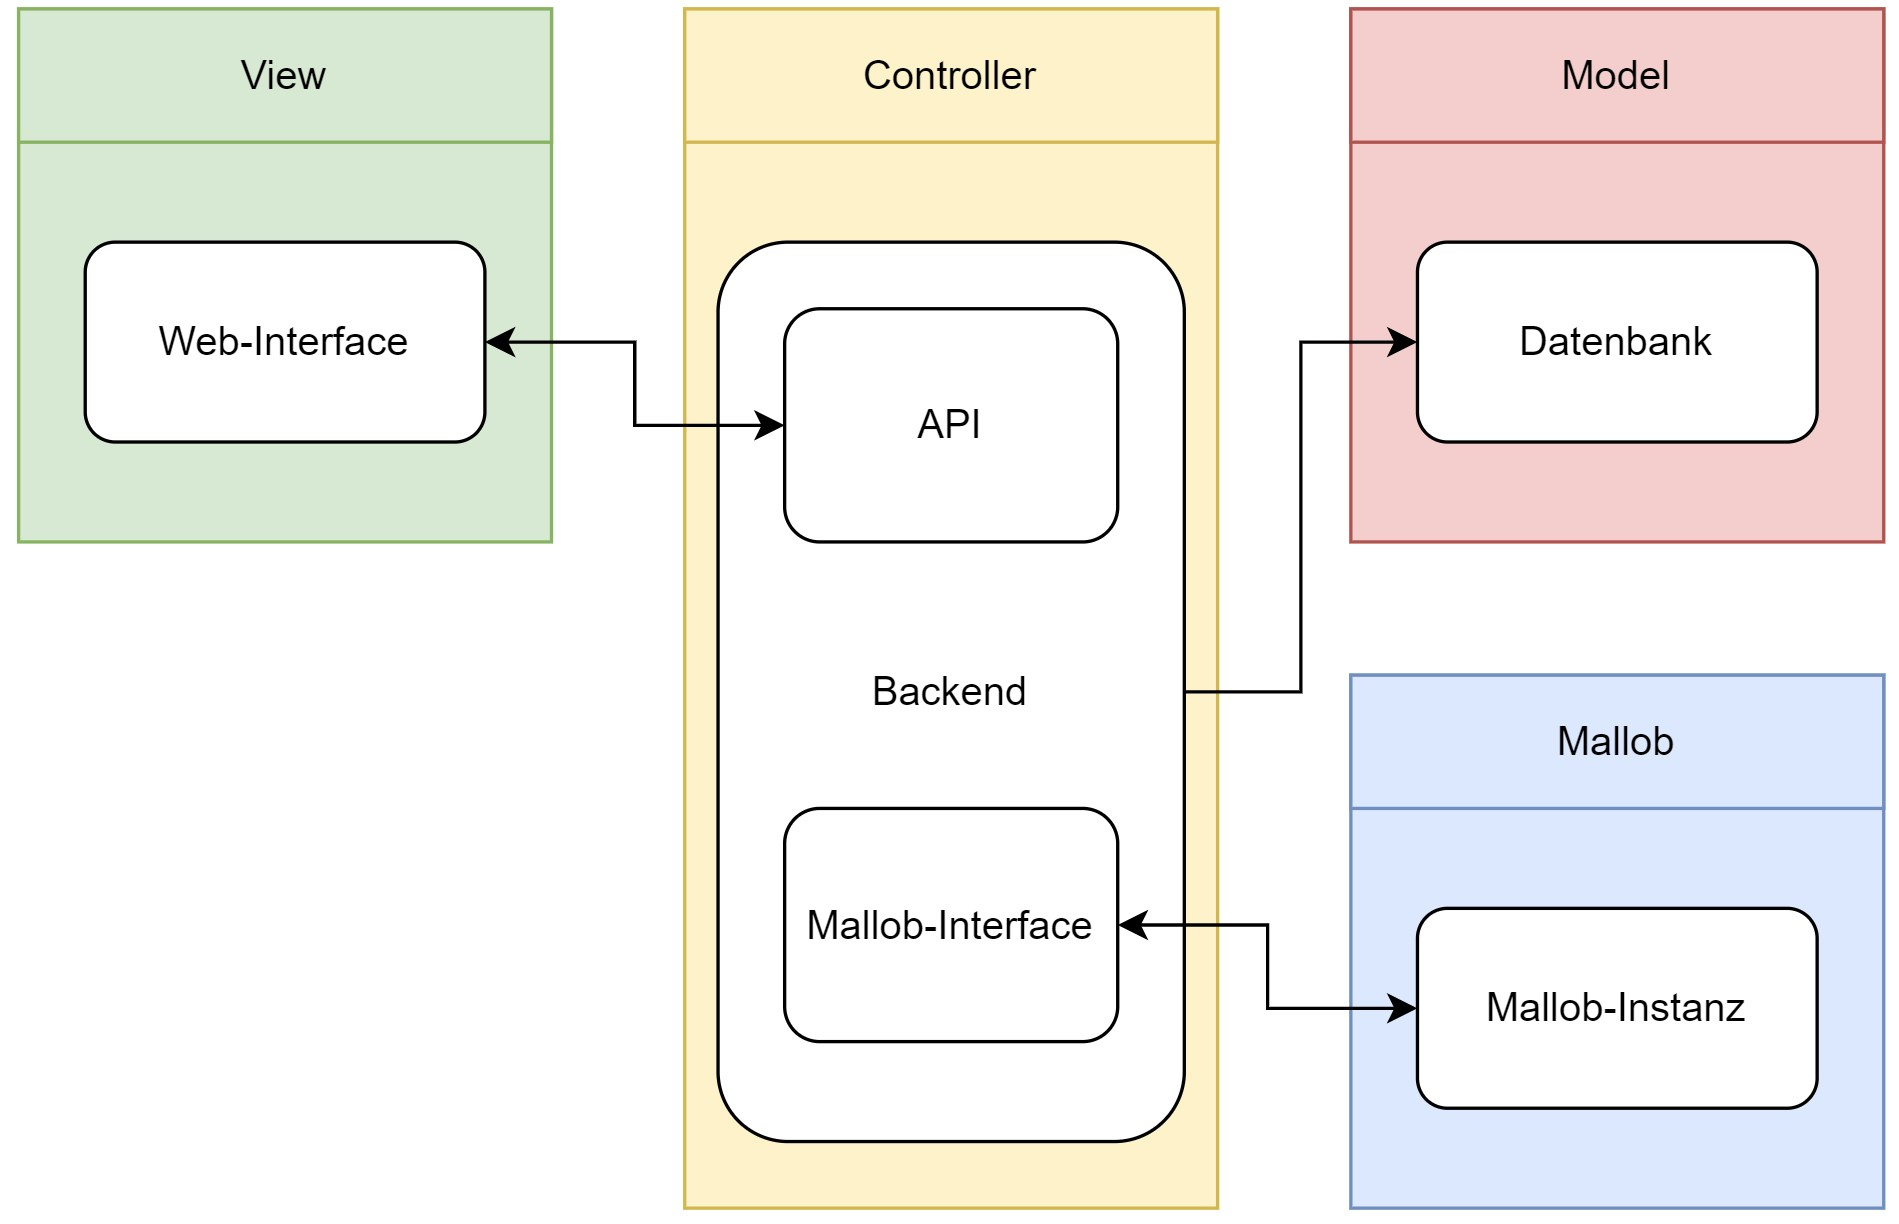
\includegraphics[width=\textwidth]{images-interface/Diagramme/Systemdiagramm3.jpg} \\
    \caption{\gls{Model-View-Controller}}
\end{figure}
Das System kann semantisch in 3 Komponenten gegliedert werden; View, Controller sowie Model. \\
Die Aufgabe des \textbf{Views}, bzw. des Web-Interfaces ist es dabei eine interaktive, grafische Benutzeroberfläche für die Interaktion mit Mallob bereitzustellen. \\
Der \textbf{Controller}, bzw. \gls{API} sowie Backend (Anfragen gehen über \gls{API} an das Backend) sind für die Kommunikation zwischen \gls{Datenbank}, Mallob und \gls{Web-Interface}, bzw. \gls{Nutzer} zuständig. Das Mallob-Interface ist im Backend implementiert und für die Kommunikation zwischen der Backend-Logik und einer laufenden Mallob-Instanz zuständig.\\
Im \textbf{Model} hält eine \gls{Datenbank} die \hyperref[PD]{Daten des Systems}. \\
\textbf{Extern} liegt die laufende Mallob-Instanz. Mallob ist nicht Teil unseres Systems. Unser System kommuniziert lediglich mit Mallob.

\pagebreak

\subsection{Anwendungsfalldiagramme}

\begin{figure}[H]
    \centering    
    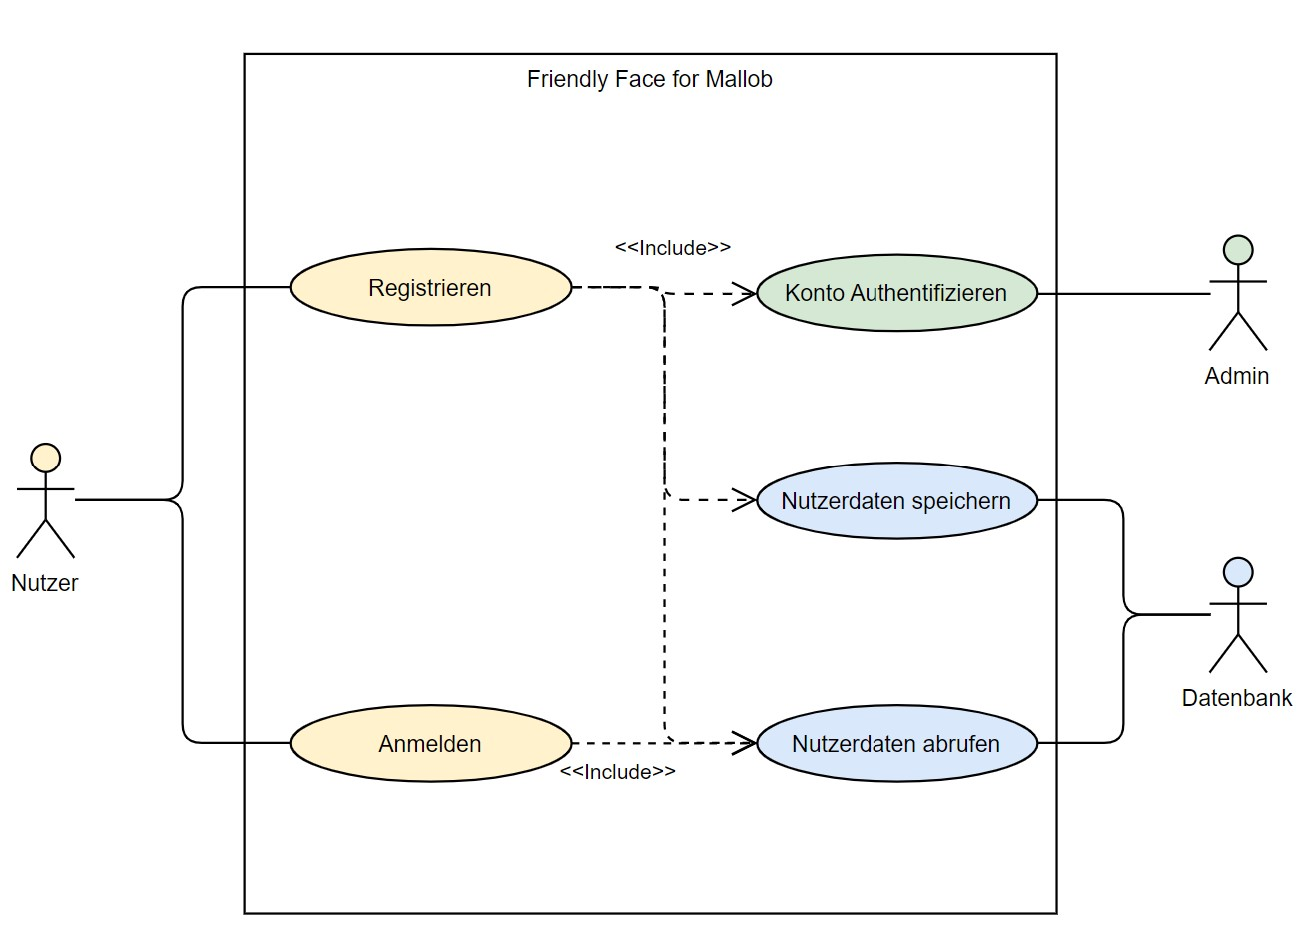
\includegraphics[width=\textwidth]{images-interface/Diagramme/Login_register_3_screenshot.jpg} 
    \caption{Registrierung von \gls{Nutzer}n}
\end{figure}


Registriert sich ein \gls{Nutzer} gemäß \hyperref[FA:API:Registrierung von Nutzern]{F1150}, so wird seine Registrierunganfrage von einem \gls{Administrator} verifiziert. Die \gls{Datenbank} speichert die \hyperref[PD:Nutzerdaten]{Nutzerdaten}.\\
Möchte sich ein registrierter \gls{Nutzer} im \gls{Web-Interface} anmelden, so werden die Nutzerdaten aus der \gls{Datenbank} geholt und mit den eingegebenen Daten verglichen.



\begin{figure}[H]
    \centering
    \includegraphics[width=\textwidth]{images-interface/Diagramme/Request_authntification_screenshot.jpg}
    \caption{Authentifizierung von \gls{API}-Anfragen}
\end{figure}
Jede Anfrage an die \gls{API} muss authentifiziert werden. Dies geschieht, indem der \gls{Authentifizierungstoken}, der mit der Anfrage geschickt wurde, mit dem in der \gls{Datenbank} gespeichertem \gls{Authentifizierungstoken} abgeglichen wird. Wurde eine Anfrage authentifiziert, also sichergestellt, das der \gls{Nutzer} diese auch ausführen darf, so wird sie weiterverarbeitet.\\
Jede Anfrage an die \gls{API} wird für eine gewisse Zeit gespeichert, um sie später noch einmal referenzieren oder einsehen zu können.

\pagebreak

%https://www.overleaf.com/project
\begin{figure}[H]
    \centering
    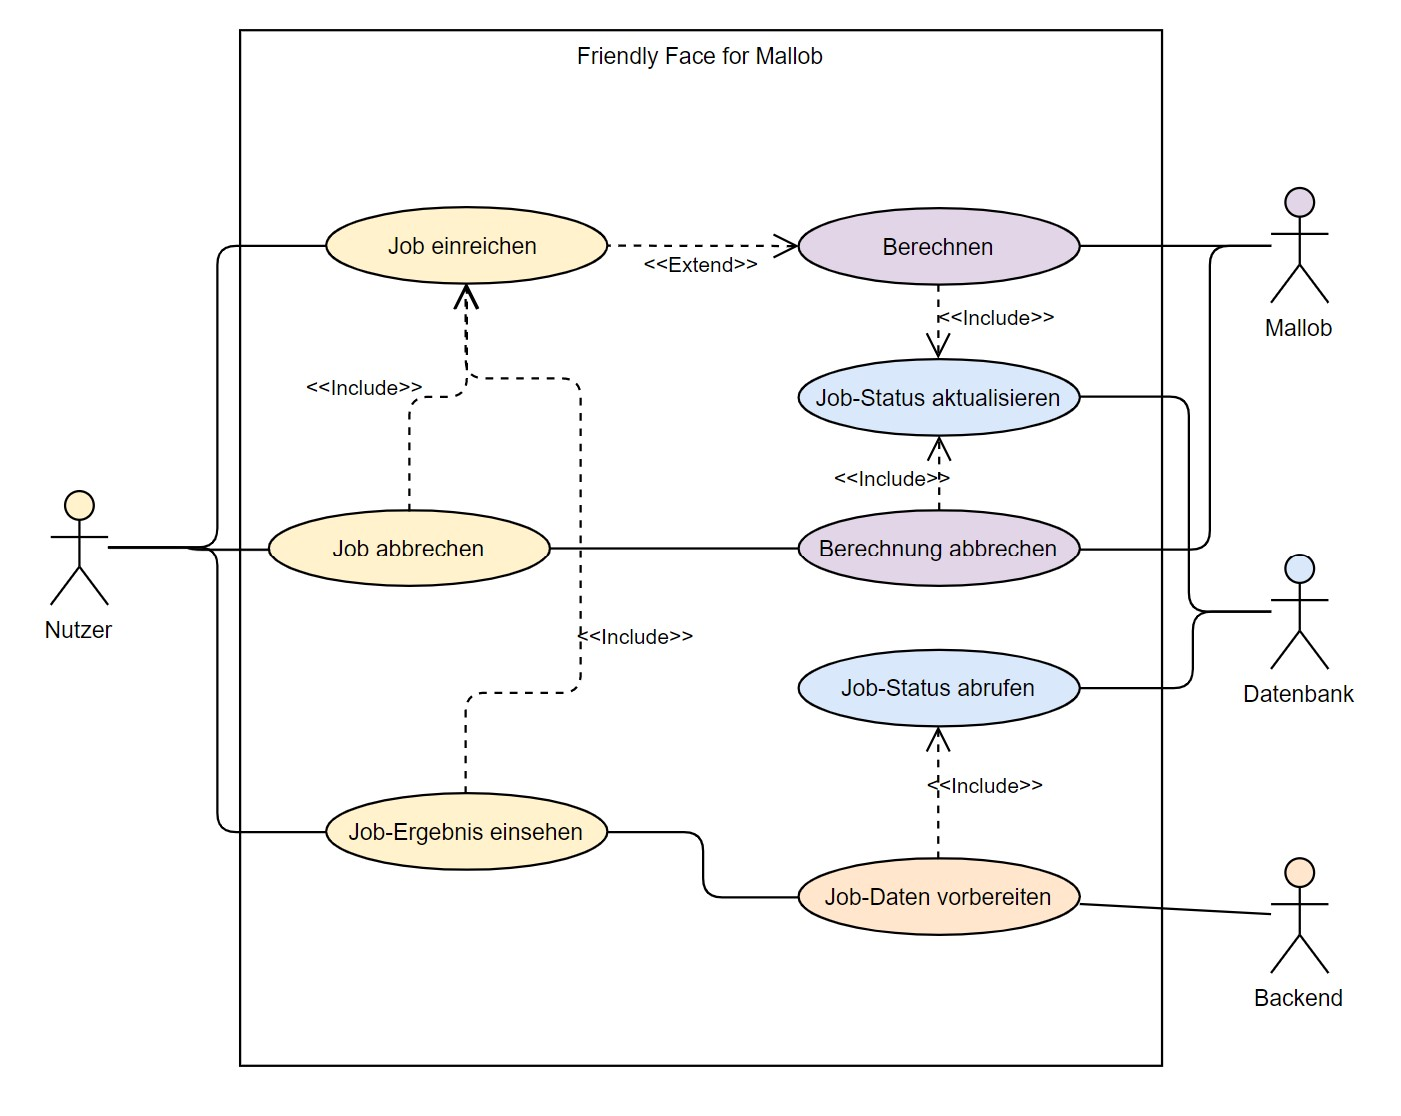
\includegraphics[width=\textwidth]{images-interface/Diagramme/Submit-abort-view-screenshot.jpg}
    \caption{Einreichen, Abbrechen und Einsehen von \hyperref[B:Jobs]{Jobs}}
\end{figure}

Reicht ein \gls{Nutzer} einen \hyperref[B:Jobs]{Job} ein, so wird dieser (je nach Konfiguration) von Mallob bearbeitet. Mallob gibt dabei Rückmeldung über den Job-Status, also entweder das \hyperref[B:Job-Ergebnis]{Ergebnis} des \hyperref[B:Jobs]{Jobs}, oder ob ein Fehler aufgetreten ist. Dieser Status wird in der \gls{Datenbank} gespeichert. \\
Ein \gls{Nutzer} kann die Bearbeitung eines \hyperref[B:Jobs]{Jobs}, der gerade von Mallob berechnet wird, abbrechen. Die berechneten Zwischenergebnisse werden dann gespeichert und können später abgerufen werden. \\
Möchte ein \gls{Nutzer} einen \hyperref[B:Jobs]{Job} einsehen, so ist es wichtig, dass dieser bereits eingereicht wurde. Um ein \hyperref[B:Jobs]{Job} einsehen zu können werden zunächst die angeforderten \hyperref[B:Job-Informationen]{Job-Informationen} aus der \gls{Datenbank} geholt und dann vorbereitet an den \gls{Nutzer} geschickt.


%\begin{center}
%    \includegraphics[scale=0.6]{images-interface/Request_authntification_screenshot.jpg} \\
%    Anwendungsfalldiagramm 2: Authentifizierung von \gls{API}-Requests
%\end{center}


\begin{figure}[H]
    \centering
    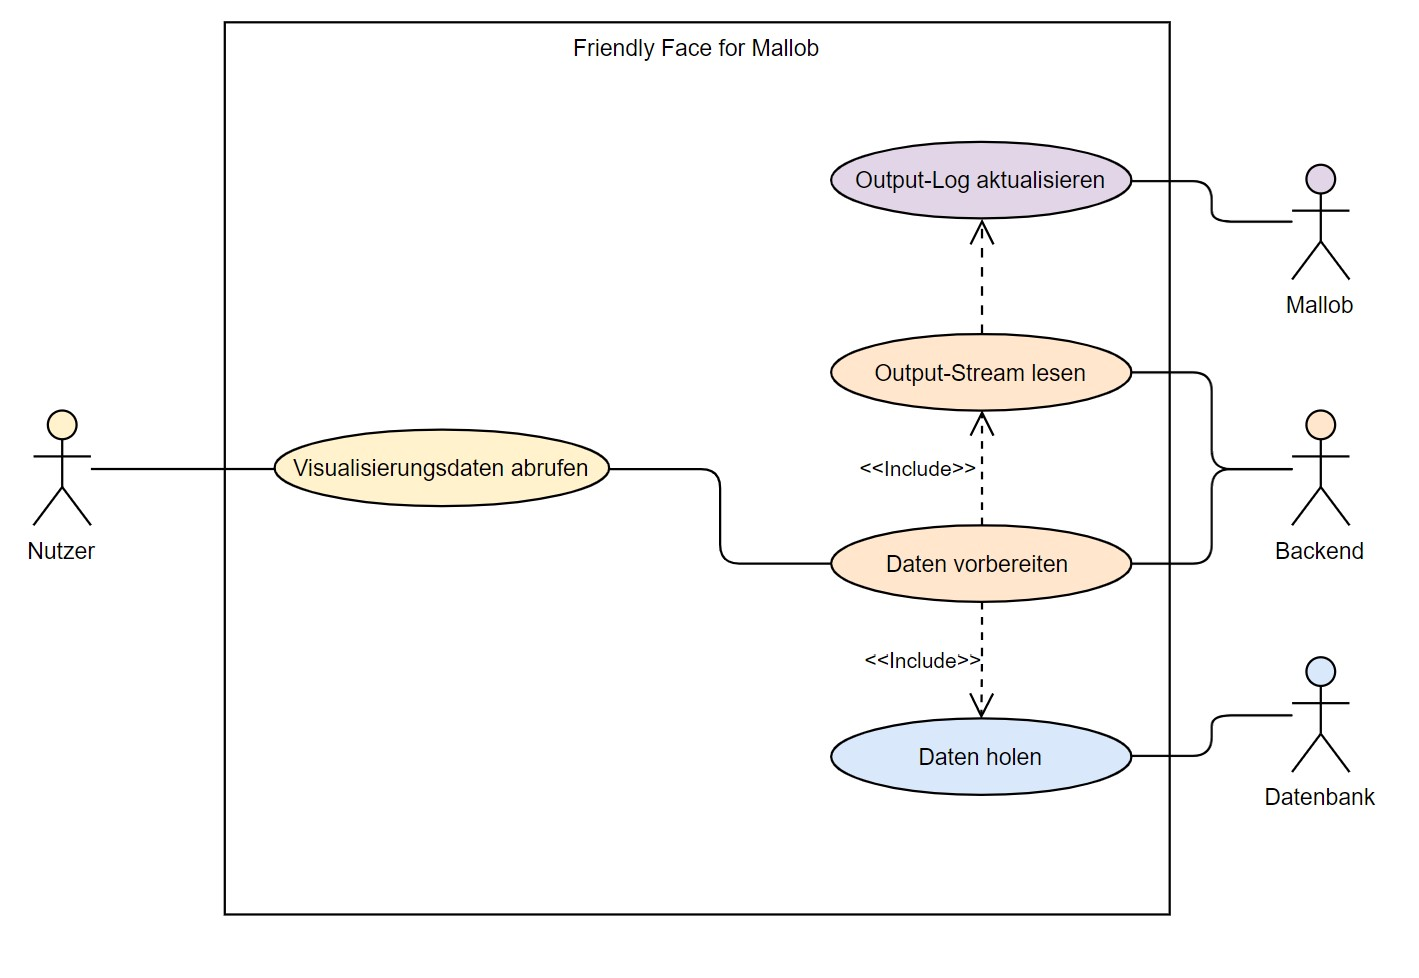
\includegraphics[width=\textwidth]{images-interface/Diagramme/visualisierungsdaten_anwendungsfaelle.jpg}
    \caption{Mallob-Visualisierungsdaten abrufen}
\end{figure}
Möchte ein \gls{Nutzer} Mallob-Visualisierungsdaten abrufen, so holt das System bereits vergangene \hyperref[B:Event]{Events} aus der \gls{Datenbank}, um daraus die Daten für die Visualisierung vorzubereiten. Des weiteren wird live der Output-\gls{Stream} der \gls{Log-Datei} von Mallob ausgelesen, um die Echtzeit-Visualisierung für den \gls{Nutzer} anzubieten. 


\pagebreak

\subsection{Aktivitätsdiagramme}
\begin{figure}[H]
    \centering
    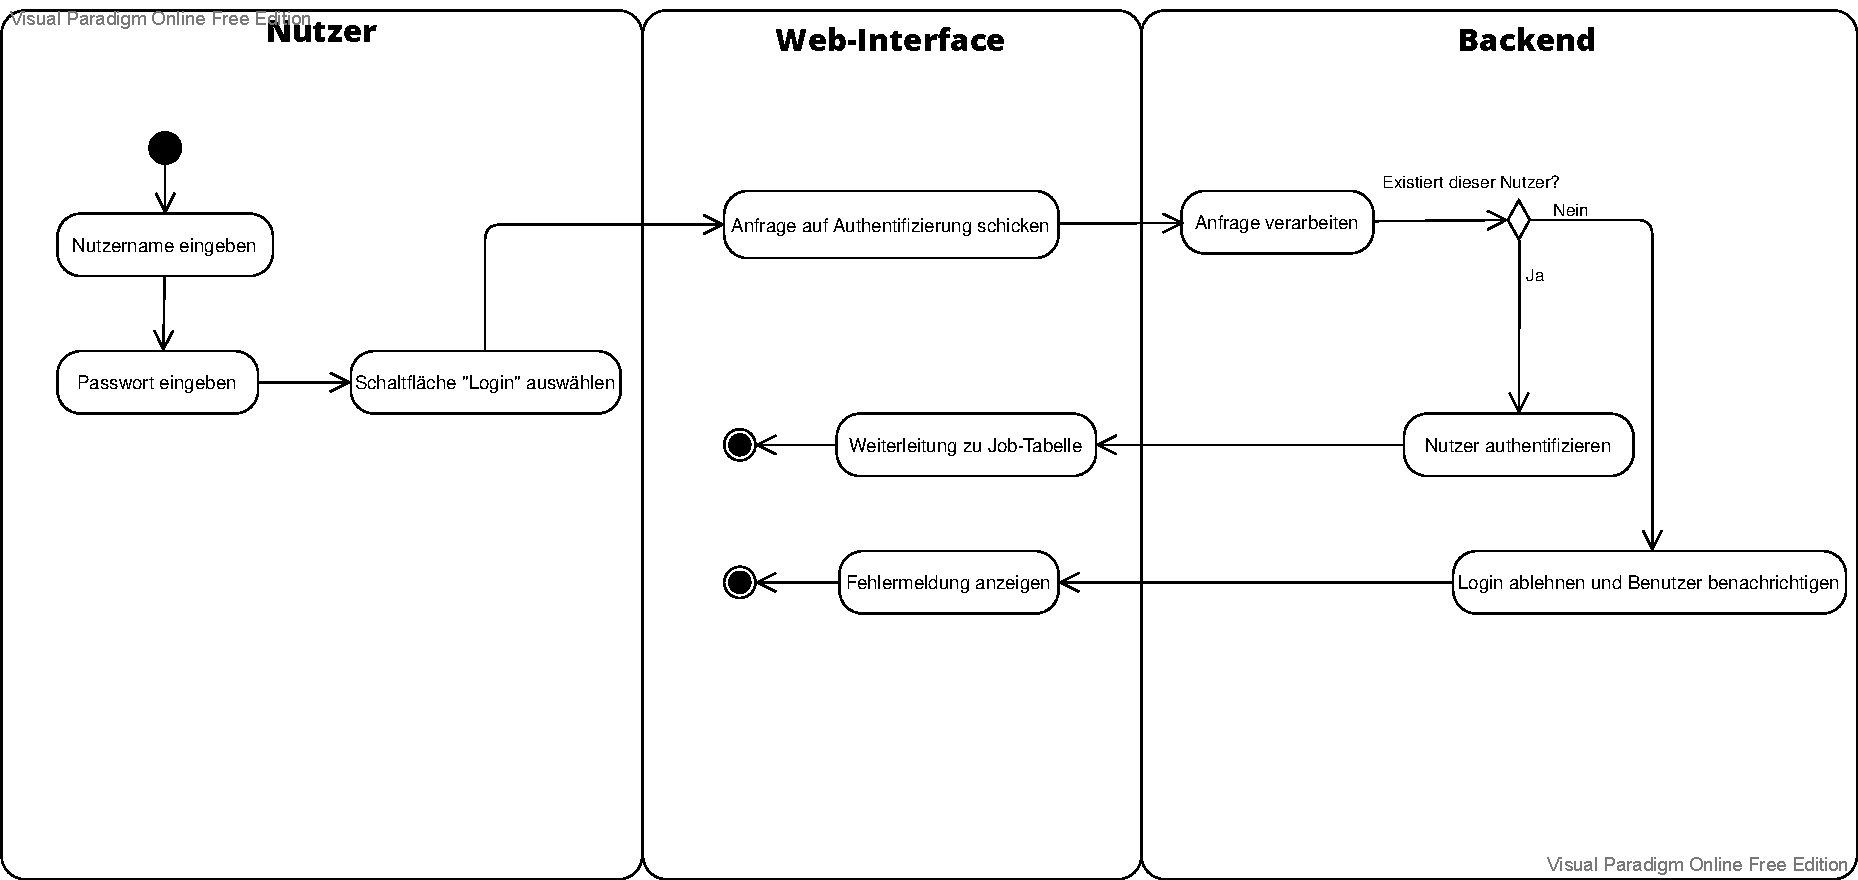
\includegraphics[width=\textwidth]{images-interface/v3_aktivitaetsdiagramme/Anmelden_v10.pdf}
    \caption{Anmeldung im System über das \gls{Web-Interface}}
    \label{fig:login_activity}
    
\end{figure}
Ein \gls{Nutzer} muss sich anmelden, um die Funktionen des \gls{Web-Interface}s zu benutzen. Zuerst gibt der \gls{Nutzer} über die Eingabe-Maske seinen Nutzernamen und Passwort ein und klickt auf die Schaltfläche \enquote{Login}, wobei das \gls{Web-Interface} seine Anfrage zur Authentifizierung an die \gls{API} schickt. Die \gls{API} überprüft die Daten und hat zwei Möglichkeiten: Entweder existiert der \gls{Nutzer} mit diesen Anmelde-Daten im System, er wird authentifiziert und das \gls{Web-Interface} leitet ihn zur \hyperref[pages:job-table]{Job-Tabelle} weiter, oder die Anmelde-Anfrage wird abgelehnt und das \gls{Web-Interface} zeigt dem \gls{Nutzer} eine Fehlermeldung.


\begin{figure}[H]
    \centering
    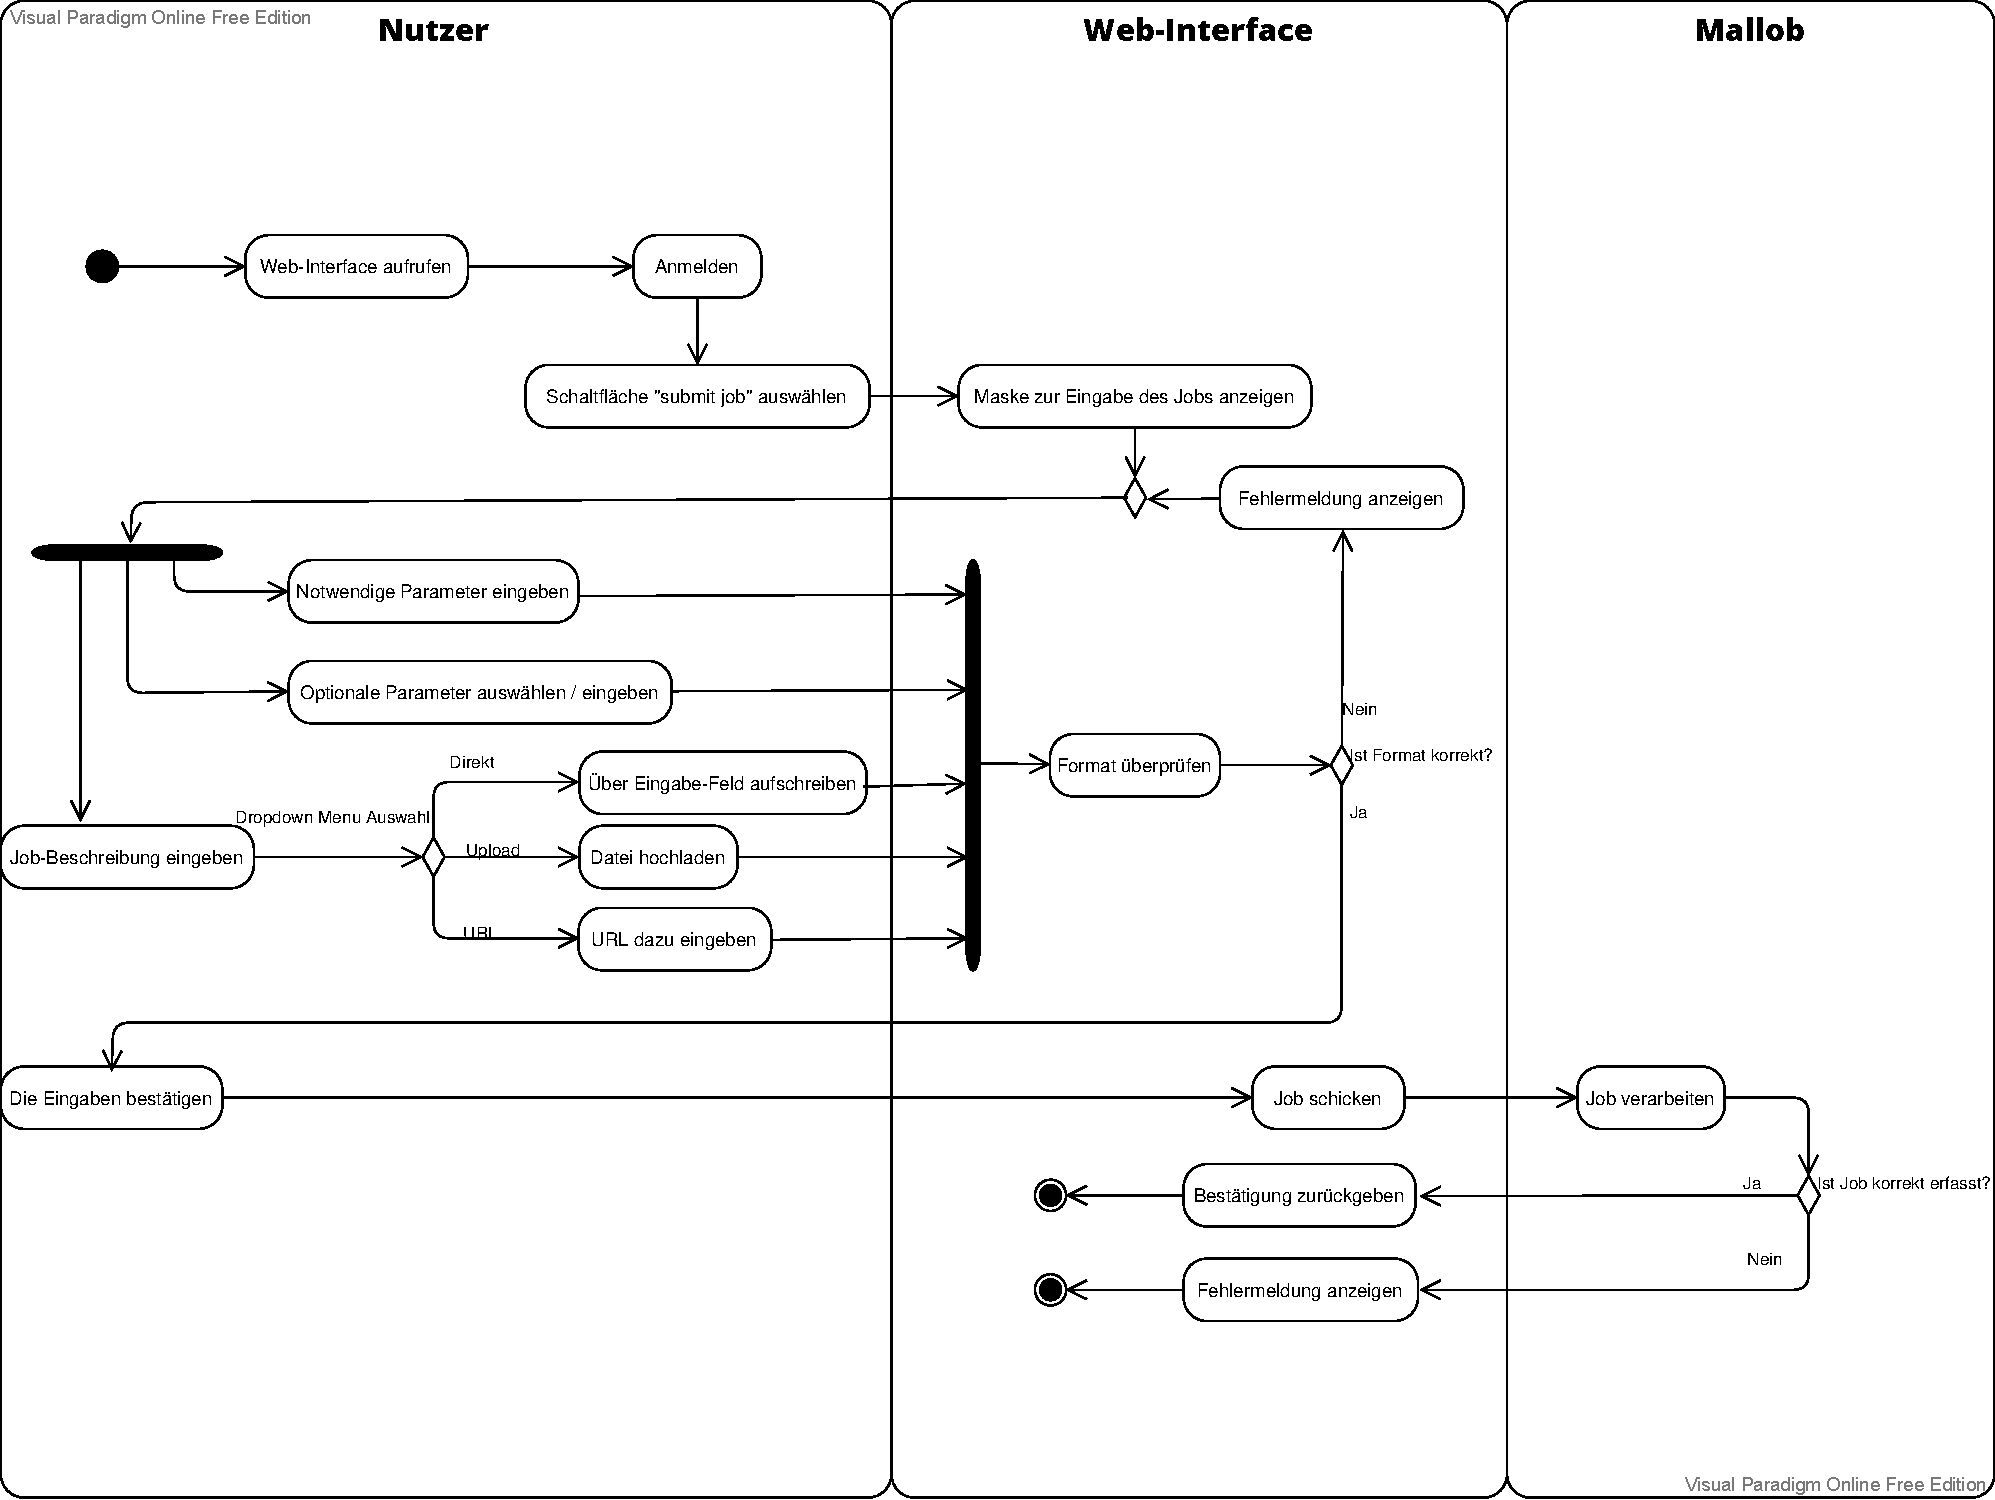
\includegraphics[width=\textwidth]{images-interface/v3_aktivitaetsdiagramme/Job_einreichen_v11.pdf}
    \caption{Einreichen eines \hyperref[B:Jobs]{Jobs} über das \gls{Web-Interface}}
\end{figure}
Möchte ein \gls{Nutzer} einen \hyperref[B:Jobs]{Job} einreichen, muss er angemeldet sein. Zunächst wählt er die Schaltfläche \enquote{submit job}. Daraufhin zeigt das \gls{Web-Interface} eine \hyperref[pages:submit-job]{Eingabe-Maske} an. Hier muss er die notwendigen Parameter eingeben, die gewünschten optionalen Parameter auswählen und die \hyperref[B:Job-Beschreibung]{Job-Beschreibung} über genau eine der drei Möglichkeiten übergeben. Über ein \gls{Dropdown-Menue}, wählt er dafür zwischen direkter Eingabe, Hochladen einer Datei, die die Beschreibung enthält oder Angabe einer URL. Nach Bestätigung der Eingabe wird das Format der Eingaben vom \gls{Web-Interface} überprüft. Falls das Format inkorrekt war, muss der \gls{Nutzer} die inkorrekte Eingabe verändern, andernfalls kann der \gls{Nutzer} die Eingaben bestätigen, was seine \hyperref[B:Jobs]{Job} über das \gls{Web-Interface} zu Mallob schickt. Mallob überprüft die \hyperref[B:Job-Beschreibung]{Job-Beschreibung} und die \hyperref[B:Job-Konfiguration]{Job-Konfiguration}. Falls diese fehlerhaft sind, wird eine Fehlermeldung vom \gls{Web-Interface} angezeigt. Falls die Daten des \hyperref[B:Jobs]{Jobs} vom \gls{Nutzer} im korrekten Format eingegeben wurden, wird eine Bestätigung zur \hyperref[B:Jobs]{Job}-Bearbeitung vom \gls{Web-Interface} zurückgegeben.

\begin{figure}[H]
    \centering
    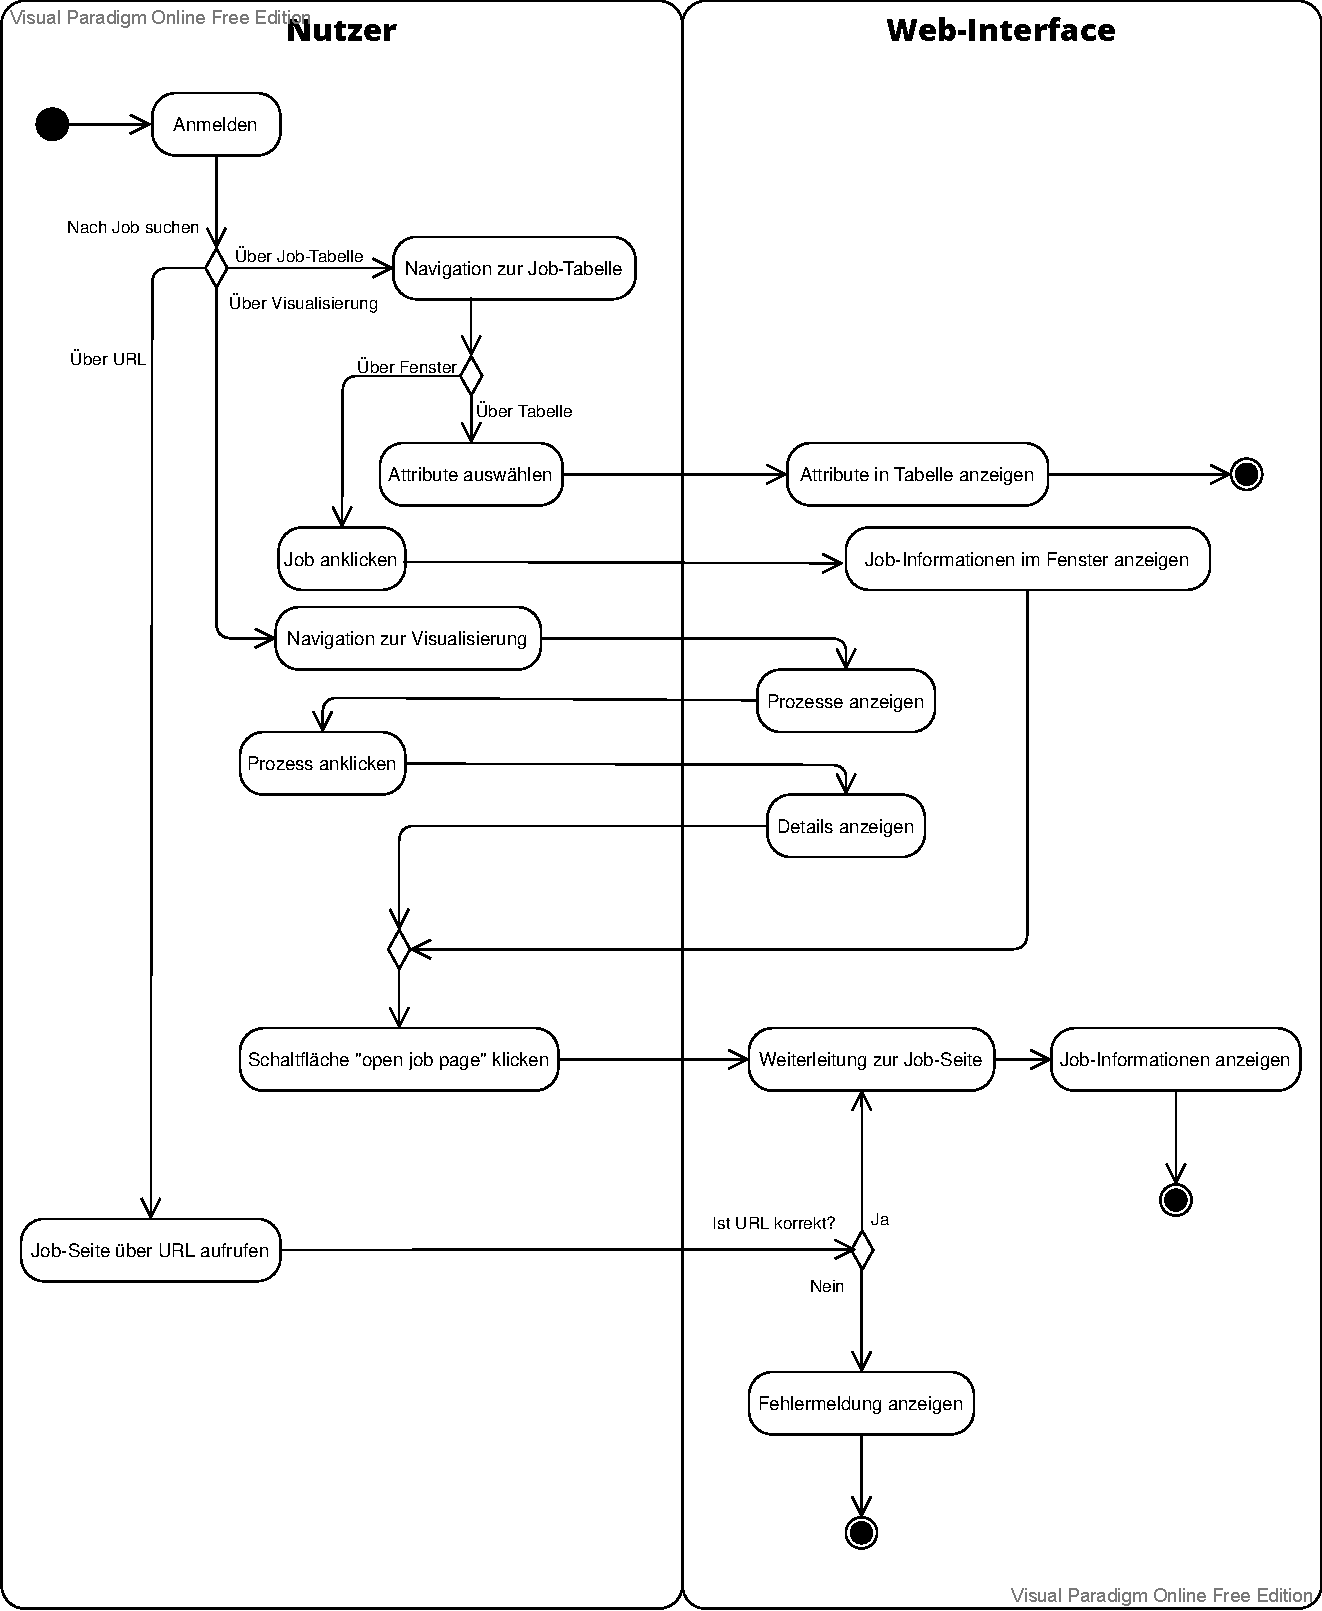
\includegraphics[width=\textwidth]{images-interface/v3_aktivitaetsdiagramme/Get_information_v3.pdf}
    \caption{Einsehen von \hyperref[B:Job-Informationen]{Job-Informationen}}
\end{figure}
\newpage
Hier werden die verschiedene Wege zum Einsehen der \hyperref[B:Job-Informationen]{Job-Informationen} angezeigt. Zuerst muss immer ein \gls{Nutzer} dafür angemeldet sein. Dann hat er 3 Möglichkeiten: 
\begin{enumerate}
   

\item Der \gls{Nutzer} gibt die URL einer Job-Seite im Browser ein und wird auf diese weitergeleitet, auf welcher ihm die \hyperref[B:Job-Informationen]{Job-Informationen} angezeigt werden.

%[TODO]  : was ist der satz bei 2.? Was ist PE
\item Der \gls{Nutzer} klickt die Schaltfläche \enquote{Visualization} an. Danach klickt er auf einen Prozess und es werden die \hyperref[B:Job-Details]{Details} dazu angezeigt. Dann klickt er auf die Schaltfläche \enquote{open job page}, was ihn zur Job-Seite weiterleitet und ihm da die \hyperref[B:Job-Informationen]{Job-Informationen} anzeigt werden.

\item Der \gls{Nutzer} navigiert zur \hyperref[pages:job-table]{Job-Tabelle}, die seine eingereichten \hyperref[B:Jobs]{Jobs} enthält. Hier kann er entweder ein Attribut aus dem \gls{Dropdown-Menue} auswählen, welches dann in der Tabelle als Spalte angezeigt wird, oder er klickt einen der angezeigten \hyperref[B:Jobs]{Jobs} an und die \hyperref[B:Job-Informationen]{Job-Informationen} werden in einem nebenstehenden Fenster angezeigt. Hier kann man ebenfalls die Schaltfläche \enquote{open job page} wählen, was ihn zu Job-Seite weiterleitet und da die \hyperref[B:Job-Informationen]{Job-Informationen} anzeigt.
\end{enumerate}
\newpage
\section{Produktleistungen}

%%
%ProduktleistungenSofern 
%an einzelne Funktionen des Programms besondere Anforderungen in Bezug auf die Zeit oder die Genauigkeit gestellt werden, sollten diese in diesem Kapitel dargestellt werden. Dabei sollten Sie prüfen, ob die zu erbringenden Leistungen mit den in Punkt 5 genannten Angaben  realisierbar sind.
%

\begin{itemize}[noitemsep]
    \item[P100] Die maximale Anzahl der \hyperref[B:Jobs]{Jobs} ist begrenzt.
    
    \item[P110] Die maximale Anzahl \hyperref[B:Jobs]{Jobs}, die ein \gls{Nutzer} gleichzeitig in Bearbeitung haben kann, ist beschränkt.
    
    \item[P120] Die Zeit, die benötigt wird, um einen beliebigen Zeitpunkt in der \hyperref[pages:visualization]{Visualisierung} darzustellen, muss linear in der Anzahl der zu ladenden \hyperref[B:Event]{Events} sein.
    
    \item[P130] (Wunschbedingung)  Die Zeit, die benötigt wird, um einen beliebigen Zeitpunkt in der \hyperref[pages:visualization]{Visualisierung} darzustellen, muss konstant sein, unabhängig vom gewählten Zeitpunkt.
    
    \item[P140] Das \gls{Web-Interface} ist auch auf kleineren Bildschirmen, wie etwa einem Handy-Bildschirm, nutzbar.
    
    \item[P150] Die \gls{Konfigurationsdatei} wird immer nur beim Systemstart eingelesen, etwaige Änderungen werden also erst mit einem Neustart des Systems wirksam.
    
    \item[P160] Beim Einreichen eines \hyperref[B:Jobs]{Jobs} im Interface erfolgt schon im Frontend eine Kontrolle der Syntax, welche den \gls{Nutzer} momentan über Fehler in der Eingabe informiert.
    
    \item[P170] Nutzernamen sind eindeutig und bestehen aus 4 bis 25 Zeichen.

    \item[P180] Passwörter müssen mindestens 8-stellig sein.
    
    \item[P190] Die gespeicherten \hyperref[B:Jobs]{Jobs} werden automatisch nach einem spezifizierten Zeitraum gelöscht.

    \item[P200] Die Größe der \hyperref[B:Job-Beschreibung]{Job-Beschreibung}, die man im \gls{Web-Interface} eingeben kann, ist beschränkt.

    
    \item[P210] Jedes \gls{Nutzerkonto} besitzt nach Registrierung die gleiche Priorität. Diese kann vom kann vom \gls{System-Administrator} geändert werden.
    
    
    \item[P220] Der \gls{Nutzer} erhält auf jede \gls{API}-Anfrage außer \hyperref[FA:API:Andauernde Abfrage des Ergebnisses eines Jobs]{F1110} unmittelbar eine  Antwort.
    
    \item[P230] Die \hyperref[pages:visualization]{Visualiseriung} ist skalierbar, sodass auch mehrere Tausend \glslink{Prozess}{Prozesse} angezeigt werden können. Um dies zu ermöglichen, wird die Qualität bei vielen \glslink{Prozess}{Prozessen} entsprechend reduziert.%, beispielsweise durch das Weglassen von Verbindungen zwischen den Prozessen.
    
    \item[P240] Daten über \hyperref[B:Jobs]{Jobs}, die nicht dem angemeldetem \gls{Nutzer} gehören, werden stets pseudonymisiert ausgegeben und dargestellt. Ist ein \gls{Administrator} angemeldet, so werden die Daten nicht pseudonymisiert.
    
    %\item[P250] Es ist möglich, die \hyperref[pages:job-page]{Job-Seite} direkt über eine passende \gls{URL} aufzurufen.
    
    \item[P260] Die maximale Geschwindigkeit der \hyperref[pages:visualization]{Visualisierung} ist das zweihundertfache.
    
    \item[P270] Die über \gls{Nutzer} gespeicherte Daten können von einem \glspl{System-Administrator} geändert werden, um beispielsweise die Priorität des \gls{Nutzer}s zu ändern oder ein \glslink{Nutzerkonto}{Konto} zu verifizieren, aber auch andere \gls{Nutzer} zum \gls{Administrator} zu machen.
    
    \item[P280] Das Backend wird in Java implementiert.

    \item[P290] Globale Einstellungen des Systems werden in einer \gls{Konfigurationsdatei} gespeichert und mit jedem Neustart aktualisiert.

\end{itemize}
\newpage
\input{9_Benutzeroberfläche}
\newpage
\input{10_Testfälle_und_Testszenarien}
\newpage
\input{11_Qualtiätsbestimmungen}
\newpage
\section{Entwicklungs-Umgebung}
        \begin{itemize}[noitemsep]
            \item Betriebssysteme 
                \begin{itemize}[noitemsep]
                    \item Windows 10
                    \item Arch Linux
                \end{itemize}
            \item Modellierung %[TODO] 
            \item Entwicklung %[TODO]
            \begin{itemize}[noitemsep]
                \item Notepad ++
            \end{itemize}
            \item Versionverwaltung
                \begin{itemize}[noitemsep]
                    \item Git
                    \item Github
                \end{itemize}
            \item Sonstige Software
                \begin{itemize}[noitemsep]
                    \item \LaTeX \hspace{0.1cm} (für das Pflichtenheft)
                    \item \href{https://de.overleaf.com}{Overleaf} (Schreiben des Pflichtenheftes)
                    \item \href{https://www.figma.com}{Figma} (GUI-Entwürfe)
                    \item \href{https://online.visual-paradigm.com/}{Infographic Maker} (Aktivitätsdiagramme)
                    \item \href{https://app.diagrams.net/}{} (Anwendungsfalldiagramme)
                \end{itemize}
        \end{itemize}   
\newpage




%---------------------------Kommunikation mit Mallob------    
%\section{Kommunikation mit Mallob}
%
%\begin{itemize}
%    \item Annahme für uns : Mallob läuft auf selben Dateisystem wie Backend 
%    \item JSON und Jobbeschreibung werden in einem Verzeichnis im Dateisystem abgelegt und von dort aus von Mallob verarbeitet
%    \item Der Output wird von Mallob ebenfalls las Datei in einem Verzeichnis ausgegeben
%    \item JSON und Jobbschreibung können unterschiedliche Dateien sein (siehe Einreichen der Jobbeschreibung, API)
%\end{itemize}









%------------------------Glossar
\newpage
\glsaddall
\setglossarystyle{altlist}
\printnoidxglossaries
\end{document}
